\documentclass[12pt]{extarticle}

\usepackage{amsmath, amsthm, amsfonts, enumitem, graphicx, subcaption, cleveref, tabularx, xpatch, imakeidx, setspace, mathptmx, titlesec, fancyhdr, etoolbox, tocloft, lipsum, amssymb, algorithm, algpseudocode, placeins, mwe, float,xcolor, listings, subfig}
\usepackage[font=small, singlelinecheck=off]{caption}
\usepackage[backend=biber,style=numeric]{biblatex}
\usepackage[a4paper,top=3cm,bottom=2.5cm,left=2.5cm,right=2.5cm]{geometry}

\definecolor{mGreen}{rgb}{0,0.6,0}
\definecolor{mGray}{rgb}{0.5,0.5,0.5}
\definecolor{mPurple}{rgb}{0.58,0,0.82}
\definecolor{backgroundColour}{rgb}{0.95,0.95,0.92}

\lstdefinestyle{CStyle}{
    backgroundcolor=\color{backgroundColour},   
    commentstyle=\color{mGreen},
    keywordstyle=\color{magenta},
    numberstyle=\tiny\color{mGray},
    stringstyle=\color{mPurple},
    basicstyle=\footnotesize,
    breakatwhitespace=false,         
    breaklines=true,
    captionpos=b,                    
    keepspaces=true,                 
    numbers=left,                    
    numbersep=5pt,                  
    showspaces=false,                
    showstringspaces=false,
    showtabs=false,         
    tabsize=2,
    morekeywords={vacancies_list},
    language=C
}

\makeindex

\addbibresource{src/bib/references.bib}

% TIPOGRAPHY
% Page settings
\pagestyle{fancy}
\fancyhf{}
\fancyfoot[C]{\thepage}

% Line spacing
\onehalfspacing

% Paragraph indent
\setlength{\parindent}{0.7cm}

% Chapter and section titles
\titleformat{\chapter}[display]{\bfseries\Huge}{\chaptername\ \thechapter}{20pt}{\bfseries\LARGE}
\titleformat{\section}{\normalfont\Large\itshape}{\thesection}{1em}{}

% Blockquote setup
\newenvironment{blockquote}{\begin{quote}\onehalfspacing\fontsize{11}{13.2}\selectfont}{\end{quote}}

% Footnotes
\renewcommand{\footnotesize}{\fontsize{10}{12}\selectfont}
\setlength{\footnotesep}{\baselineskip}
\appto\footnotesize{\singlespacing}

% CUSTOM COMMANDS
\newcommand{\meqref}[1]{Eq.\ref{#1}}
\newcommand{\mfigref}[1]{Fig.\ref{#1}}
\newcommand{\mtabref}[1]{Tab.\ref{#1}}
\newcommand{\mappendixref}[1]{Appendix \ref{#1}}
\newcommand{\indfunc}[1]{\textit{\textbf{1}}_{#1}}
\newcommand{\midcaption}[1]{
    \captionsetup{justification=centering}
    \caption{#1}
}
\makeatletter
\xpatchbibmacro{textcite}{%
  \printnames{labelname}%
}{%
  \printfield[citetitle]{labelname}%
}{}{}


\newbibmacro{aycite}{%
\textit{
  \defcounter{maxnames}{1}%
  \ifnameundef{labelname}
    {\printfield{labeltitle}%
     \setunit{\printdelim{nonameyeardelim}}}
    {\printnames{labelname}%
     \setunit{\printdelim{nameyeardelim}}}
  \printtext[bibhyperref]{\printlabeldateextra}%
	{(\printfield{year})}%
	\textsuperscript{\printfield{labelnumber}}
  }}

\DeclareCiteCommand{\fancycite}
  {\usebibmacro{prenote}}%
  {\usebibmacro{citeindex}%
   \usebibmacro{aycite}}
  {\multicitedelim}
  {\usebibmacro{postnote}} 

\DeclareCiteCommand{\ucite}
  {\usebibmacro{prenote}}
  {\textsuperscript{\textit{\printfield{labelnumber}}}}
  {\multicitedelim}
  {\usebibmacro{postnote}}
\makeatother

\begin{document}


\begin{titlepage}
    \begin{center}
        
\includegraphics[height=3.6cm]{./src/imgs/unimib_logo_2.png}
        \vspace*{1.45cm}

        \Large
        {Submitted to Department of Informatics, Systems and Communication (DISCo), Bachelor's Degree in Computer Science, in association with Department of Physics "Giuseppe Occhialini"}

        \vspace*{1.5cm}
        
        \Huge
        \textbf{Properties and Implementation of Sequential Expansion of Latin Hypercube Sampling for Simulation Design}

        \normalsize
        \vspace*{2cm}

        \begin{minipage}[t]{0.47\textwidth}
	       {Supervisor:} \vspace{0.3em} \\
              {\large \textbf{Prof. Davide Gerosa}} \vspace{1em}  \\
              {Co-supervisor:} \vspace{0.3em} \\
              {\large \textbf{Prof. Davide Elio Ciucci}}\\
              {Co-supervisor:} \vspace{0.3em} \\
              {\large \textbf{Dott. Matteo Boschini}}
        \end{minipage}
        \hfill
        \begin{minipage}[t]{0.47\textwidth}\raggedleft
	       {Authored by:} \hspace{-0.9em} \vspace{0.3em} \\
              {\large \textbf{Alessandro Crespi}}
              {\footnotesize student number 879186}
        \end{minipage}

        \vfill
        Academic year 2023/2024
            
    \end{center}
\end{titlepage}

\tableofcontents
\pagebreak

\begin{abstract}
%\textit{Stochastic methods are key techniques for consuming computational-demanding simulations because they handle complex systems with many variables, thanks to their high scalability, where deterministic methods fail short or are impractical. However, the latter guarantee much more result stability. Latin Hypercube Sampling, which belongs to the quasi-Monte-Carlo category, takes the best of either stochasticity and deterministic approaches: it draws random sampling of a model's parameter hyperspace but belonging to pre-determined specific intervals, or strata. Such a property is called stratification. This research seeks to horizontally scale an already instanced LHS distribution, which is hardly possible, and simultaneously maintaining stratification as much as possible. Such a technique, namely `expanded Latin Hypercube Sampling` (eLHS), aims to give LHS-based simulations more flexibility over the next stages of an evolutionary simulation apparatus. Evolutionary apparatus are involved when a simulation run is consumed but the resulting surrogate model is not eligible for experiments, thus the simulation must resume. The eLHS algorithm, wrapped and distributed under the authors' package `latinexpansion` for Python, allows the user to expand a hyperparameter set and it gives the experimenter the opportunity of controlling other desired  properties.}
\textit{Stochastic methods are crucial for managing computationally demanding simulations because they effectively handle complex systems with many involved variables, offering high scalability where deterministic methods fall short. On the other hand, deterministic methods cut result variance. Latin Hypercube Sampling (LHS), a quasi-Monte Carlo technique, combines the benefits of both stochastic and deterministic approaches. It draws random samples from a model’s parameter space within predetermined specific intervals, or strata, a property known as stratification. This research aims to horizontally scale an existing LHS distribution while maintaining stratification as much as possible, a challenging task. The proposed technique, named expanded `Latin Hypercube Sampling` (eLHS), enhances the flexibility of LHS-based simulations in the later stages of an evolutionary simulation process. Evolutionary apparatus are involved when a simulation’s surrogate model is insufficient for experiments, requiring the simulation to continue. The eLHS algorithm, available in the authors’ Python package `latinexpansion`, allows users to expand a hyperparameter set and provides control over other desired properties.}
\end{abstract}


\section{Introduction}
Simulation design is a branch of Statistics focused on building better simulations to enhance the comprehension of phenomena. These simulations are widely used in mathematics, physics, economics, mechanics, and other scientific fields as tools for proving theories, interpolating real sampled values, and generating predictive models to explore uncharted traits and features, perhaps intuitively or roundly developed in the early stages of the study of a specific problem.

Since the advent of hybrid mechanical-electrical programmable calculators such as IBM's machines, the first of their kind to be really useful in engineering, scientists have used them to perform heavy computations for experiments. In 1969, Kennar and Stone's Computer Aided Design for Experiments (CADEX)\ucite{kennard1969} proposal for computer-driven experiments led to spread up a broad variety of Computer-based simulation methods.

Eventually, computer-based simulations are a set of strategies that benefit from mathematical modeling techniques based on discrete known points placed in a limited parameter space, hereafter samples, and the computer programmability advantage has been used to design, shape and enhance a specific subset of samples that satisfies the desired properties, hereafter sample sets. 

The general concept of computer simulation has been defined in the past few decades, it's based on the following key ideas: taking into account a desired behavior $ F $ the experimenters have an interest in, F has to be explored through its $ P $ real parameter space; the algorithm takes samples from a standard $ NP $-dimensional hyperspace $ \Omega $ and arranges the sample set for the simulation; afterwar, the simulation is carried out by evaluating $ F $ over the sample set and eventually producing a so-called surrogate model. The class of algorithms meant to implement this abstraction is commonly labeled with \textit{sampling methods}.

To the category of sampling methods belongs the fixed-step (or determined-step) samplers, which include a $h(x)$ function that evenly space samples across the hyperspace or somehow deterministically. For instance, consider $h(x)$ constant function or a Chebyshev nodes \ucite{stewart1996}. For the matter of this paper, we have focused on the sampling methods whose points are drawn with a specific random distribution.

A critical consideration when evaluating sampling methods is the trade-off between exploration and exploitation. An exploration-oriented sample set maximizes the simulation expertise of seeking key features over the studied behavior. Exploration has been depicted as a model-free practice, so that it does not base its own actions on the model (behavior) evolution or any other on-site response. On the other hand, exploitation is an auxiliary mechanism that aims to better assist the simulation by deploying samples in strategic placements that prevent exploration from exceeding the prediction surrogate made upon a key region (such as overshooting an optima or mismatching a discontinuity for a steep slope).

The most iconic sampling method for simulations is the pseudo-random sampling, lightened of every other criteria, namely the Monte Carlo Sampling or MCS (\fancycite{metropolis1987})  which has been outlined as basic design of sampling methods. Quasi-Monte Carlo methods are a class of sampling algorithms based on Monte Carlo, indeed, but without a proper random drawing of sample points from the parameter space, instead, points are sequentially extracted in order to satisfy one or multiple criteria as best as the computational time required remains acceptable. Many criteria have been theorized and tested; each of them has a proper application context.

In the scope of this matter, the authors will focus on the space-filling class of criteria and, particularly, on the stratification procedure (also known as non-overlapping property); The former measures the quality of a sample set to be spread evenly across an hyperspace; the way space-filling is defined determines the final aspect of the sampling. On the same hand, a sample set, in $P$-dimensional space, admits the non-collapsing property if and only if the projections of the samples on a specific dimension fall into distinct intervals $I_i$. These $I_i$ intervals are fixed-width slices of the limited volume of parameter space taken into examination (e.g., an hyper-volume $[0,1)^N$) and the number of intervals is equal to the number of samples. So, the non-overlapping property prevents samples to fall into a busy area (which has been occupied by another sample). Furthermore, given that the number of intervals and the size of the sample set is equal, it does ensure there are no empty intervals across the parameter space. This property is widely known because it is the fundamental property which Latin Hypercube Sampling sets (LHS) are based on, topic of this paper.

The authors used to work with sampling methods for simulation design, more likely LHS designs \ucite{gerosa2022} \ucite{gerosa2018}, in Astrophysics related experiments, such as simulating black hole binary mergers, which obviously requires a massive amount of computational time and many different parameters. The authors often experienced difficulties predicting how long it would take to run a full simulation given $N$ known sampling points in a $P$-dimensional space. This situation forces them to reserve more machine time on a shared company supercomputer for experiments than they really need. In order to better spend the reserved machine time left after the execution of the first run of sampling points, the authors designed an algorithm that adds up points to the initial LHS sample set using another one that has been drawn by the expansion algorithm in order to preserve stratification of both sample sets together.\\
Differently, they have experienced another issue related to the accuracy of the surrogate model, result of the simulation consumed after the LHS set. Sometimes, it just happens that the model does not satisfy an eventual accuracy threshold. Instead of throwing the simulation away and compute another one, they would like to expand the current initial set with additional points to aid, the updated model, converging.

The authors of this paper propose a algorithm called \textit{Expansion of an LHS} that, indeed, takes a already existing Latin Hypercube sample set and propose a new set of points samples in the same parameter hyperspace which are supposed to maintain properties stability altogether.
The original sample set is referred as \textit{starting set} and the add-on samples as \textit{expansion set}. The whole sample set joined together by both is called \textit{expanded set}.

The paper is structured as follows: \cref{sec:lhs} yields a Latin Hypercube Sampling brief history and formal definition; in \cref{sec:lhs_expansion} is shown the research results and discussion of the expansion task issued; \cref{sec:experiments} contains experimental and example assessments on the applied expansion algorithm; \cref{sec:code_implementation} the C module package code implementation; and \cref{sec:conclusions} held the conclusions.

\section{Latin Hypercube Sampling}
\label{sec:lhs}
\subsection{What is an LHS?}
\label{subsec:what_is_an_lhs}
According to the Handbook of Combinatorial Designs \ucite{colbourn2006}, the first appearance in history of the "Latin Square" has to be attributed to the Korean mathematician Choi Seok-jeong, who described it, using modern terminologies, as a $N \times N$ matrix with $N$ distinct symbols, appearing $N$ times each but precisely once per type for each row and column. The suffix "Latin" has been inspired by the efforts that Leonhard Euler has put into this topic while defining a general theory for Latin Squares \ucite{euler1776} and using Latin letters as symbols to fill the square up with. See Fig.1 for an example with 4 objects.

\begin{figure}[h]
    \centering
    \begin{subfigure}[b]{0.45\textwidth}
        \centering
        \vtop{
        	\vspace{0pt}
        	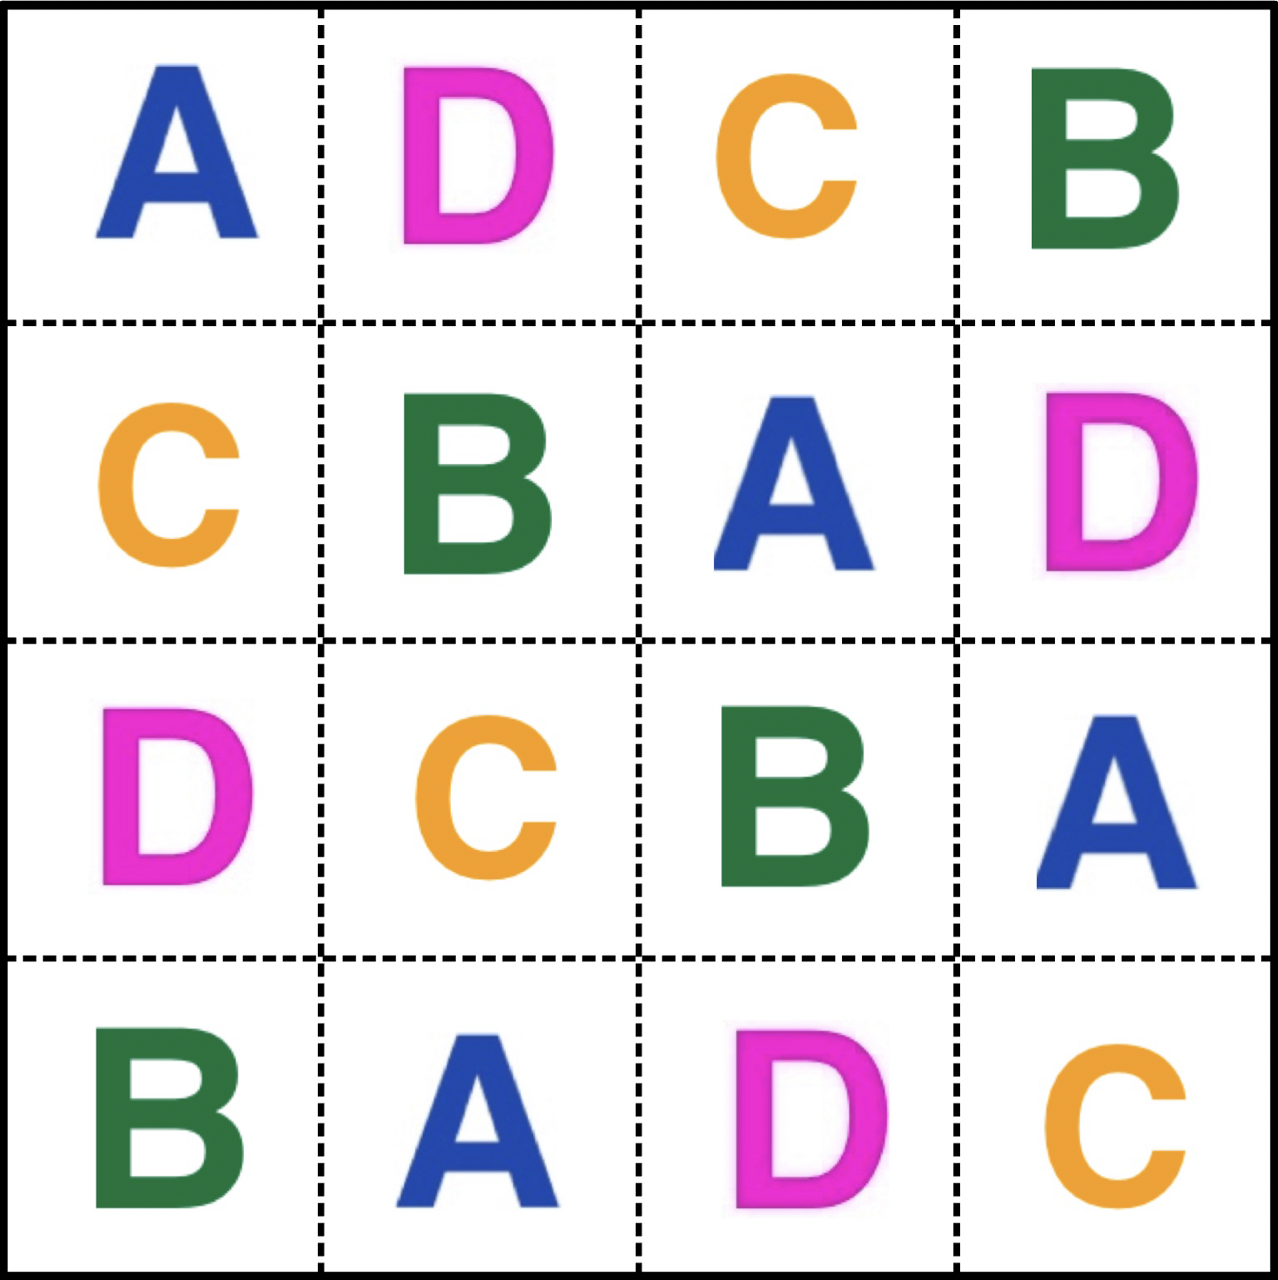
\includegraphics[width=\textwidth]{src/imgs/latin_square_letters_and_colours.png}
        	%\captionsetup{}
        	\caption{A Latin 4x4 Square with 4 distinct symbols, both letters and colors either, arranged so that no letter occurs more than once in a row or a column}
        	\label{fig:latin_square_a}
        }
    \end{subfigure}
    \hspace{0.05\textwidth}
    \begin{subfigure}[b]{0.45\textwidth}
        \centering
        \vtop{
        	\vspace{0pt}
        	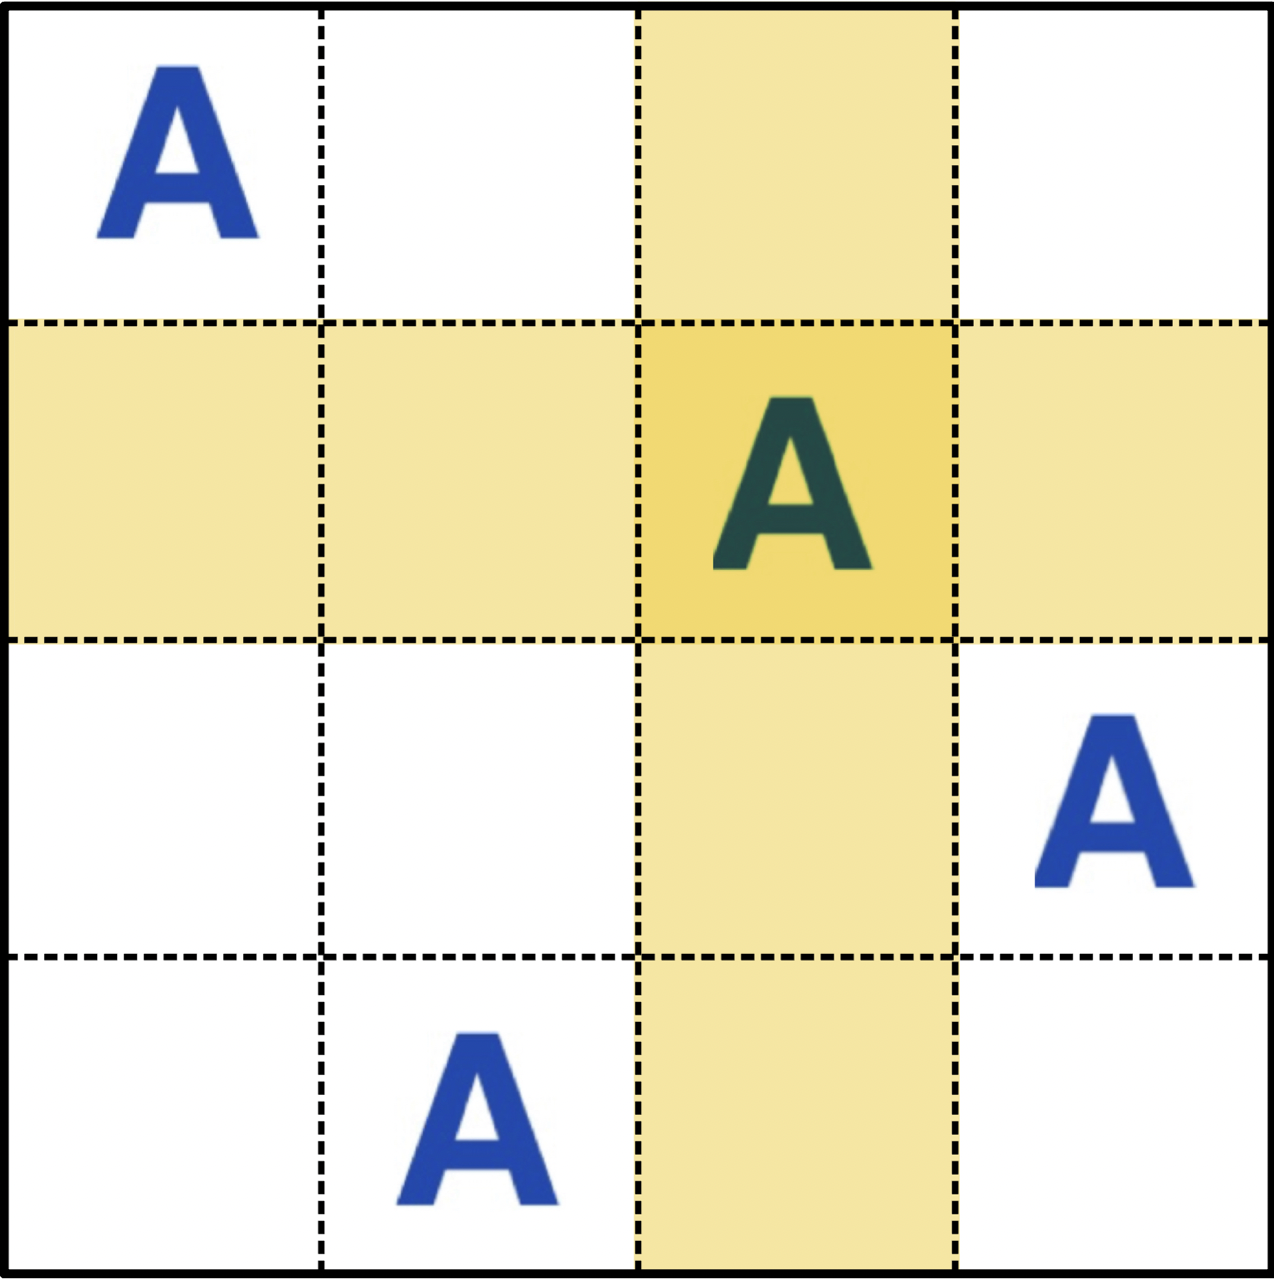
\includegraphics[width=\textwidth]{src/imgs/latin_square_skeleton.png}
        	\caption{The skeleton of (a) Latin Square highlighting only the As (or BLUE) symbol positions, it's easily noticeable how the positions does not overlap onto each other's row and column both}
        	\label{fig:latin_square_b}
        }
    \end{subfigure}
    
    \midcaption{}
    \label{fig:latin_square}
\end{figure}

In the scope of this paper, which does not aim to study combinatorial properties of $N$ symbols, we consider the placement of a sample set, which has to well stratifies the matrix. The symbols must occur in the matrix exactly $N$ times each. Instead of consider all symbols, we will look to a single one only. 

Generally, we can speak of modern Latin Hypercube designs as the Euler's Latin Square's matrix concept (depicted as a grid in Fig.1b) but deeming a more complex multidimensional matrix. $N$ symbols are placed in the same way of earlier: each symbol lies exactly once on each fiber (in literature, a "fiber" of a multidimensional matrix is the general term for a one-dimensional substructure in any dimension [or mode] of a tensor. e.g. In a 2D matrix, the fibers of the first and second dimensions are respectively "rows" and "columns").
Moreover, LHS is no longer supposed to place symbols in matrices but, instead, put $N$ random samples on a sectioned hyperspace, whose sections are familiar with the matrix's fibers. The \textit{hyperspace} represents the examined multi-parameter space of the interested model, whereof each axis is associated with a different parameter.

By definition of LHS, the parameter hyperspace has a limited span, which is the hyper-volume $[0,1)^P$, commonly used in literature. However, some texts use a different standard, and they let the parameter space take place in a $[-1,1)^P$ hypercube. Every parameter axis is sliced into smaller consecutive intervals of width $\frac{1}{N}$ that consequently depict the sub-region where each coordinate of the points is sampled randomly. In anticipation for further definitions, we provide a indexing system for intervals; in any dimension of the hypercube with $N$ intervals, for each $i$ from 0 to $N-1$, the i-th interval's boundaries are:
\begin{equation}
\label{eq:interval_index}
I_i = \Big[\frac{i}{N}, \frac{i + 1}{N}\Big)
\end{equation}
for further usage, the right term $\frac{i + 1}{N}$ of the interval was called \textit{frontier of the i-th interval} which is shared with the left hand term of $I_{i+1}$. 
With no loss of generality, the examples and considerations designed by the authors of this paper assess the random distribution to be uniform in all intervals. The uniformly distributed samples can be transformed by associated transformation functions for any other distribution (e.g. Gaussian distribution).

\subsection{How to build a Latin Hypercube Sample Set}
\label{subsec:how_to_lhs}
In this section it has been marked out mathematically the construction of an LHS sample. This description is widely used for introducing the topic on many textbooks and lectures and it takes inspiration from the work of X.Kong at al.\ucite{kong2017}.
Let $S = \{S_1, S_2, ..., S_N\}$ be the Latin Hypercube sample set with $N$ number of samples, where $\|S_i\| = P$ number of dimensions. It is comfortable to use the matrix notation $S_{ij}$, whereof rows are the i-th sample and columns, instead, represents the projection of every sample on each j-th dimension. Then, we introduce the sorted index matrix $A = \{a_{ij} = i\}$ of $N \times P$ dimension as a tool for trace the intervals index, its purpose will be clearer soon. \\
Given an $A$ index matrix, the preliminary design matrix S is given by: 

\begin{equation}
\label{eq:Sij_def}
S_{ij} = \frac{u_{ij} + a_{ij} - 1}{N}
\end{equation}

where $u_{ij}$ is a uniform distributed variable U[0,1). This preliminary design has the peculiarity to have the samples always placed on the diagonal of the hypercube $[0,1)^P$ (\mfigref{fig:diagonal_poor_design}). Now, the indexes matrix comes into use, typically shuffling the original $A$ we attain $B = \{b_{ij}\}$ random permutation, which plugging it  into \cref{eq:Sij_def} describe the uniform random variable $S_{ij}$ living inside the statistical bin identified by the interval index $b_{ij}$. We explicitly write down the uniform random variable $S_{ij}$ involving \cref{eq:interval_index} boundaries for the ij-th interval as well: 
\begin{equation}
\label{eq:rand_variable_Sij}
S_{ij} \text{ $\sim$ } U\Big[\frac{b_{ij} - 1}{N}, \frac{b_{ij}}{N}\Big)
\end{equation}

Along this paper, the authors have used the notation $R \in MC(N, P)$ that implies the $R$ be a Monte-Carlo sample set, then of $N$ points in $P$, hence $R$ is a Monte-Carlo sample set. \\
Similarly, the expression $S \in LHS(N, P)$ states that $S$ is a Latin Hypercube sample set of the same parameters.
By definition of LHS, which stress that it is a quasi-Monte-Carlo sample set distribution, we can write that:

\begin{equation*}
LHS(N, P) \; \subset \; MC(N, P)
\end{equation*}

\subsection{Degree of a Sample Set}
\label{subsec:lhs_degree}
For the purpose of this research, the authors introduced a tool to measure how much a Monte Carlo sample set is close to a Latin Hypercube one, namely \textit{degree of a sample set} with $\mathcal{D}$ identifier. This metric (\meqref{eq:degree}) is designed to assign to a sample set $S$ of $N$ elements in $P$ dimensions an index that ranges from the worst possible distributions of points when approaching 0 (it happens if samples overcrowd into the same very intervals and let many more empty) to a fully conventional LHS when degree equals to 1, such that:

\begin{equation}
\label{eq:degree_range}
0 < \mathcal{D}(S) \leq 1 \;,\; S \in MC(N,P)
\end{equation}
\\
such that
\\
\begin{equation}
\label{eq:degree_of_lhs}
\mathcal{D}(S) = 1 \;\Leftrightarrow \; S \in LHS(N, P)
\end{equation}
\\
The degree formula cast the arithmetical average of the presence (with numerical value 1) of the projection of every sample in each interval for each dimension:

\begin{equation}
\label{eq:degree}
\mathcal{D}(S) = \frac{\sum^P_{j=1}\sum^N_{q=1} min(\sum^N_{i=1}\indfunc{[\frac{q-1}{N}, \frac{q}{N})}(S_{ij}), 1)}{P \cdot N}
\end{equation}

where $\indfunc{}$ is the indicator function (see \mappendixref{appendix:indicator_function}), the variable $q$ is another way to represent the sorted index matrix $A = \{a_{ij} = i \}$ for a more immediate comprehension. The $min$ operator states that the presence of several samples' projections in a specific interval $q$ does not weight up the whole term, which would be at most 1 even if multiple samples lie in $q$. Hence, the degree formula ignores the overlapping samples onto the same interval, hereafter only \textit{overlaps}.

\subsection{Additional properties}
\label{subsec:lhs_properties}
In this section, the authors present some very important additional properties that could greatly improve the accuracy - or the quality in other terms - of the surrogate model produced by the consumed simulation.

A well known issue with LHS designs is well depicted in \mfigref{fig:diagonal_poor_design}. It's obvious that it must be considered a poor simulation design for the most of the experiments. Usually, implementations of LHS add some peculiar properties to the design. We can highlight two superclasses of properties which LHS may be joined with: model-free properties and model-based properties.


\begin{figure}[h]
    \centering
    \begin{subfigure}[b]{0.45\textwidth}
        \centering
        \vtop{
        	\vspace{0pt}
        	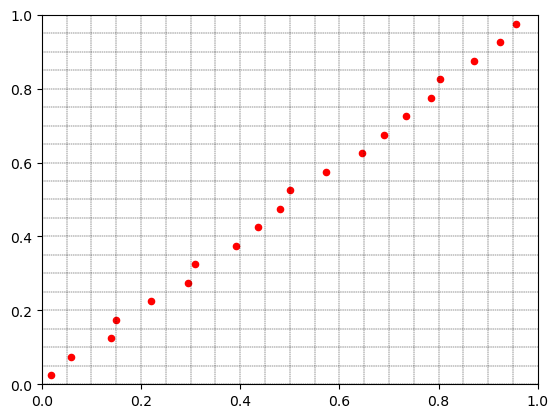
\includegraphics[width=\textwidth]{src/imgs/diagonal_poor_design.png}
        	\caption{A poor Latin Hypercube sampling in 2 dimension. Despite it stratifies completely the square, it busts the experiment parameter space.\\ The diagonal sampling depicts how insufficient a pure LHS is to achieve a good simulation.}
        	\label{fig:diagonal_poor_design}
        }
    \end{subfigure}
    \hspace{0.05\textwidth}
    \begin{subfigure}[b]{0.45\textwidth}
        \centering
        \vtop{
        	\vspace{0pt}
        	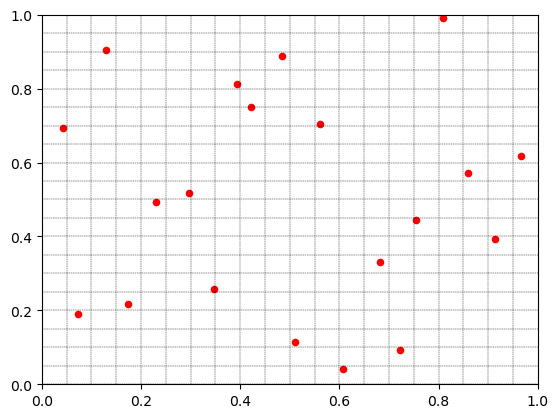
\includegraphics[width=\textwidth]{src/imgs/good_design.png}
        	\caption{LHS with space-filling property prevents samples to cluster together, low-discrepancy reduces unintentional patterns. This sampling has been generated using scipy.stats.qmc.LatinHypercube utility class. The sample generator bears random permutations of coordinates to lower the centered discrepancy \ucite{scipy2020}.}
        	\label{fig:good_design}
        }
    \end{subfigure}
    
	\midcaption{}
    \label{fig:latin_square}
\end{figure}

\subsubsection{Model-free and model-based simulation designs}
\label{subsubsec:model_free_model_based}
As the names may suggest, the latter implies the experimental design to involve some the peculiarities of the function to evaluate e.g. the shape that is expected, the initial or boundaries conditions, any well known critical region. Given that this approach is knowledge-driven, "What do we already know about?", can knock down pretty much the computational time required for the whole experiment with eventually high accuracy, but it can be equally easy that results may be biased, based on assumptions that may prove wrong later, or make hard any further effort from other scientists to retake the experiment and confirm the results if the assumptions are not completely clear.
On the other hand, the model-free is the formal way to depict a fully independent sampling of the parameter space from the experiment which it has been designed for. Because of not many criteria have been left, all of the properties in this class are based on inter-element relationships, which convey that for each of them has a heuristic meant to quantify how much each sample is well-placed among the others. The shorthand for such a class of criteria is \textit{space-filling properties}.

Beside the many interesting considerations and suggestions that the model-based class of criteria has to offer to mathematicians, the space-filling properties has highly excited the experimenter community through the decades, producing creative and curious features that the samples could experience among each others. A well-known criteria is, for instance,the maximum minimum distance among points, so-called maximin distance criterion, and its typical counterpart that minimize the maximum hole, so-called maximin distance. The assumed metric is the $P$-dimensional Euclidean distance in the hyperspace.

By the way, the characteristic non-overlapping property of the LHS itself is actually a space-filling property. It ensures that, for example, the average distance between the consecutive projections of a group of 3 samples on the same axis is at least 1/2 distance units and at most 3/2 d.u.

\subsubsection{On the optimal search tree}
\label{subsubsec:search_trees}
Despite the ease to describe a criteria for a set of elements, for instance the maximin distance, generating from random drawn a quasi-optimal solution is a nowdays a very serious issue to deal with. Actually, the algorithm should \textit{seek} for the best candidate among a broad pool of possibilities.

In Computer Science, all the possible variants of a decision-demanding problem is mapped in a search tree, a graph-based structure that is explored by querying at each node which subpath should the algorithm undertake \ucite{jacobs2010}. Some trivial well-defined path search algorithm adopts a nice binary search tree solution which, in the worst setups, is solved in linear time $O(n)$\fancycite{daskalakis2007}. However, many other undeterministic, or let's say stochastic, algorithms are easily NP-complete problem, in their average-case. Such that is the synonym of computational-demanding algorithm for non-binary search trees. Some solution was proposed by John McCarthy, and then commented by \fancycite{knuth1975}, namely the Alpha-Beta pruning algorithm which, in short, when the algorithm deepen and evaluate the tree branches it overestimates the current solution found at some extent, in the end the algorithm cuts off a lot of branches deemed not useful anymore. Alpha and Beta are two hyper-parameters that ponders the current solution value.

\section{Expansion of a Latin Hypercube Sampling}
\label{sec:lhs_expansion}
The LHS paradigm allows to implement several criteria over a rigorous grid, which forms the basis for the sequential creation of samples. Thus it's frequently utilized in engineering environments for surrogate manufacture of complex systems - see also \cref{subsec:lhs_properties}. For example, the LHS is used in hyperparameter tuning/optimization of Machine Learning models (\fancycite{koch2018}), environmental and water system analysis (\fancycite{sheikholeslami2017}), structural reliability analysis (\fancycite{olsson2003}).

There are ongoing efforts to improve the LHS capability. As previously stated, add criterions first. Then, by rethinking the foundations of the algorithm. The reader has to acquaint that Latin Hypercube technique, widely implemented, is labeled as a \textit{one-stage} algorithm in literature. The fact that all samples are distributed and assessed "on the first run" bestows this adjective. It is relevant to clear out that the actual creation and propagation of points is not properly implemented as the resulting of a single sampling random variables in agreement with \meqref{eq:rand_variable_Sij}, but instead it is a sequential drawing of points - or, possibly, a parallel drawing of several ones for optimization reasons - given a desired $N_1$ number of samples, the newest one has to be pulled out from a pool of optimal candidates in order to improve the criteria applied, such as maximin space-filling distance (see \cref{subsubsec:model_free_model_based}). The feature "one-stage" highlights that it could be possible to have many more "stages" of the algorithm. It's a game of perspectives: inside a current stage, the policy for drawing a fixed number of data points is aimed at pulling out point given the other ones; instead, a multistage policy is related to a more evolutionary approach, aiming to enhance the sample set stage by stage. Manipulating an already instantiated LHS may sound difficult because LHS is not designed to add points - or, at least, it is not supposed to consider it. Indeed, it is reasonable to assess that by adding points, one by one, over a full grid of $N_1$ intervals of an LHS, and then reshaping such a grid in $N_2 > N_1$ intervals, will lead to collisions (overlaps), which represents an issue - see \cref{subsec:multistage_task}.

The process that embodies the evolution from a precursor LHS to his next-stage has been called \textit{Expansion} by the authors; the resultant of the expansion process is the so-called \textit{expanded set}. Please refer to \mfigref{fig:algo} for the visual explanation of expansion.

Along this section, the authors used to refer several times to the expansion process without precising how the new samples are going to be placed, the actual process is described in section \cref{subsubsec:algorithm}.

\subsection{The task of multistaging sampling}
\label{subsec:multistage_task}
The multistage approach raises concerns regarding the consistency of the non-collapsing property, which is valid for one-staged setups. \mfigref{fig:example_overlaps} depicts an experiment carried out upon scipy's $S \in LHS(N_1 = 10, P = 2)$ with samples displayed over its appropriate grid of $N_1$ intervals per dimension (\mfigref{fig:example_overlaps1}). The experiment consists in evaluating the behavior of the fixed $S$ sample set while the grid is "growing" - intended as creating a brand new grid with  a greater number of intervals - one by one for three times. 
Light grey-colored rows and columns are vacant, meaning that no projections are located there; rows and columns marked in red indicate the location of overlaps. After the first add-on (\mfigref{fig:example_overlaps2}), the grid shows two overlaps in row \#3 and in column number \#3 as well; the next stage (\mfigref{fig:example_overlaps3}) shows overlaps too, four in total, more than before. In the end, \mfigref{fig:example_overlaps4} has no overlaps at all. The distribution of occurrences of overlaps when the grid grows, depends on the initial sample set. The authors discuss about this topic later in \cref{sec:experiments} [$\longleftarrow$ be more specific].

Regarding the LHS directive, the multistage experiment proposed shows that growing the interval grid could lead to downgrade the stratification in some extent (\mfigref{fig:example_overlaps2} and \mfigref{fig:example_overlaps3}) or give a new opportunity to fill the new empty space with a set of brand new samples without compromise the whole set optimality. 

\begin{figure}[]
    \centering
    \begin{subfigure}[b]{0.49\textwidth}
        \centering
        \vtop{
        	\vspace{0pt}
        	\captionsetup{skip=0pt}
        	\midcaption{}
        	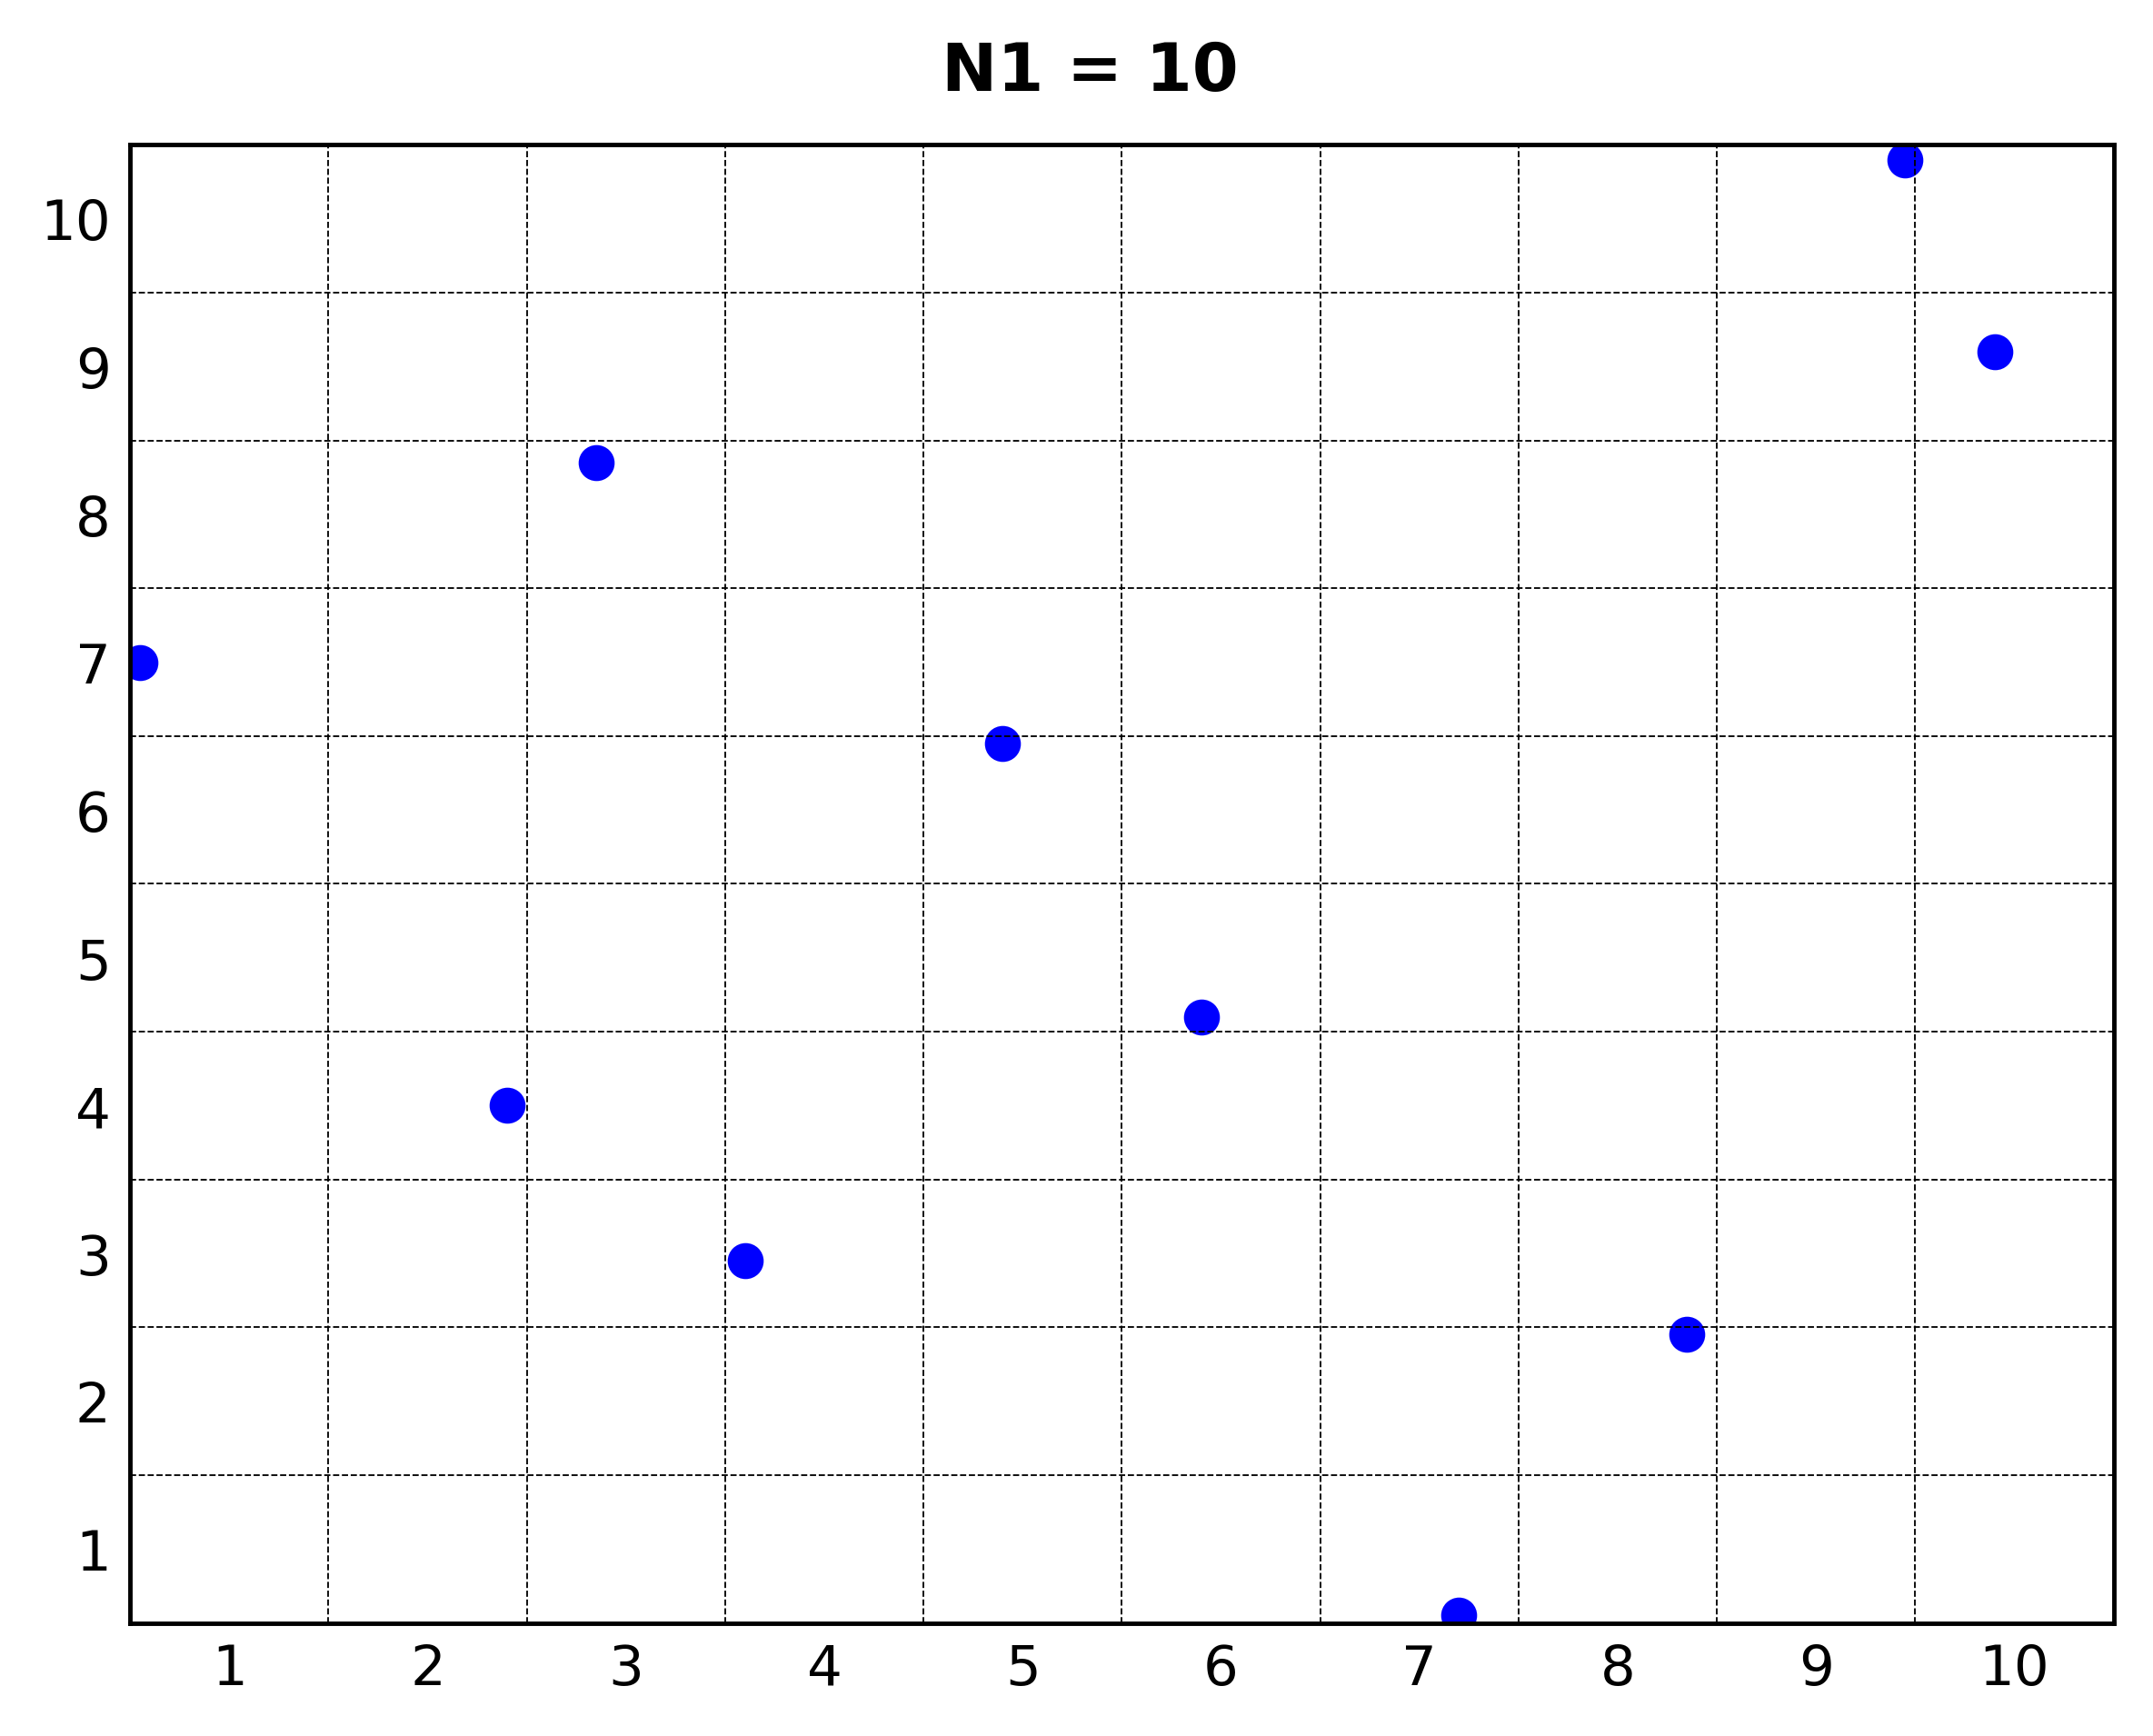
\includegraphics[width=\textwidth]{src/imgs/example_overlaps1.png}
        	\label{fig:example_overlaps1}
        }
    \end{subfigure}
    %\hspace{0.05\textwidth}
    \begin{subfigure}[b]{0.49\textwidth}
        \centering
        \vtop{
        	\vspace{0pt}
        	\captionsetup{skip=0pt}
        	\midcaption{}
        	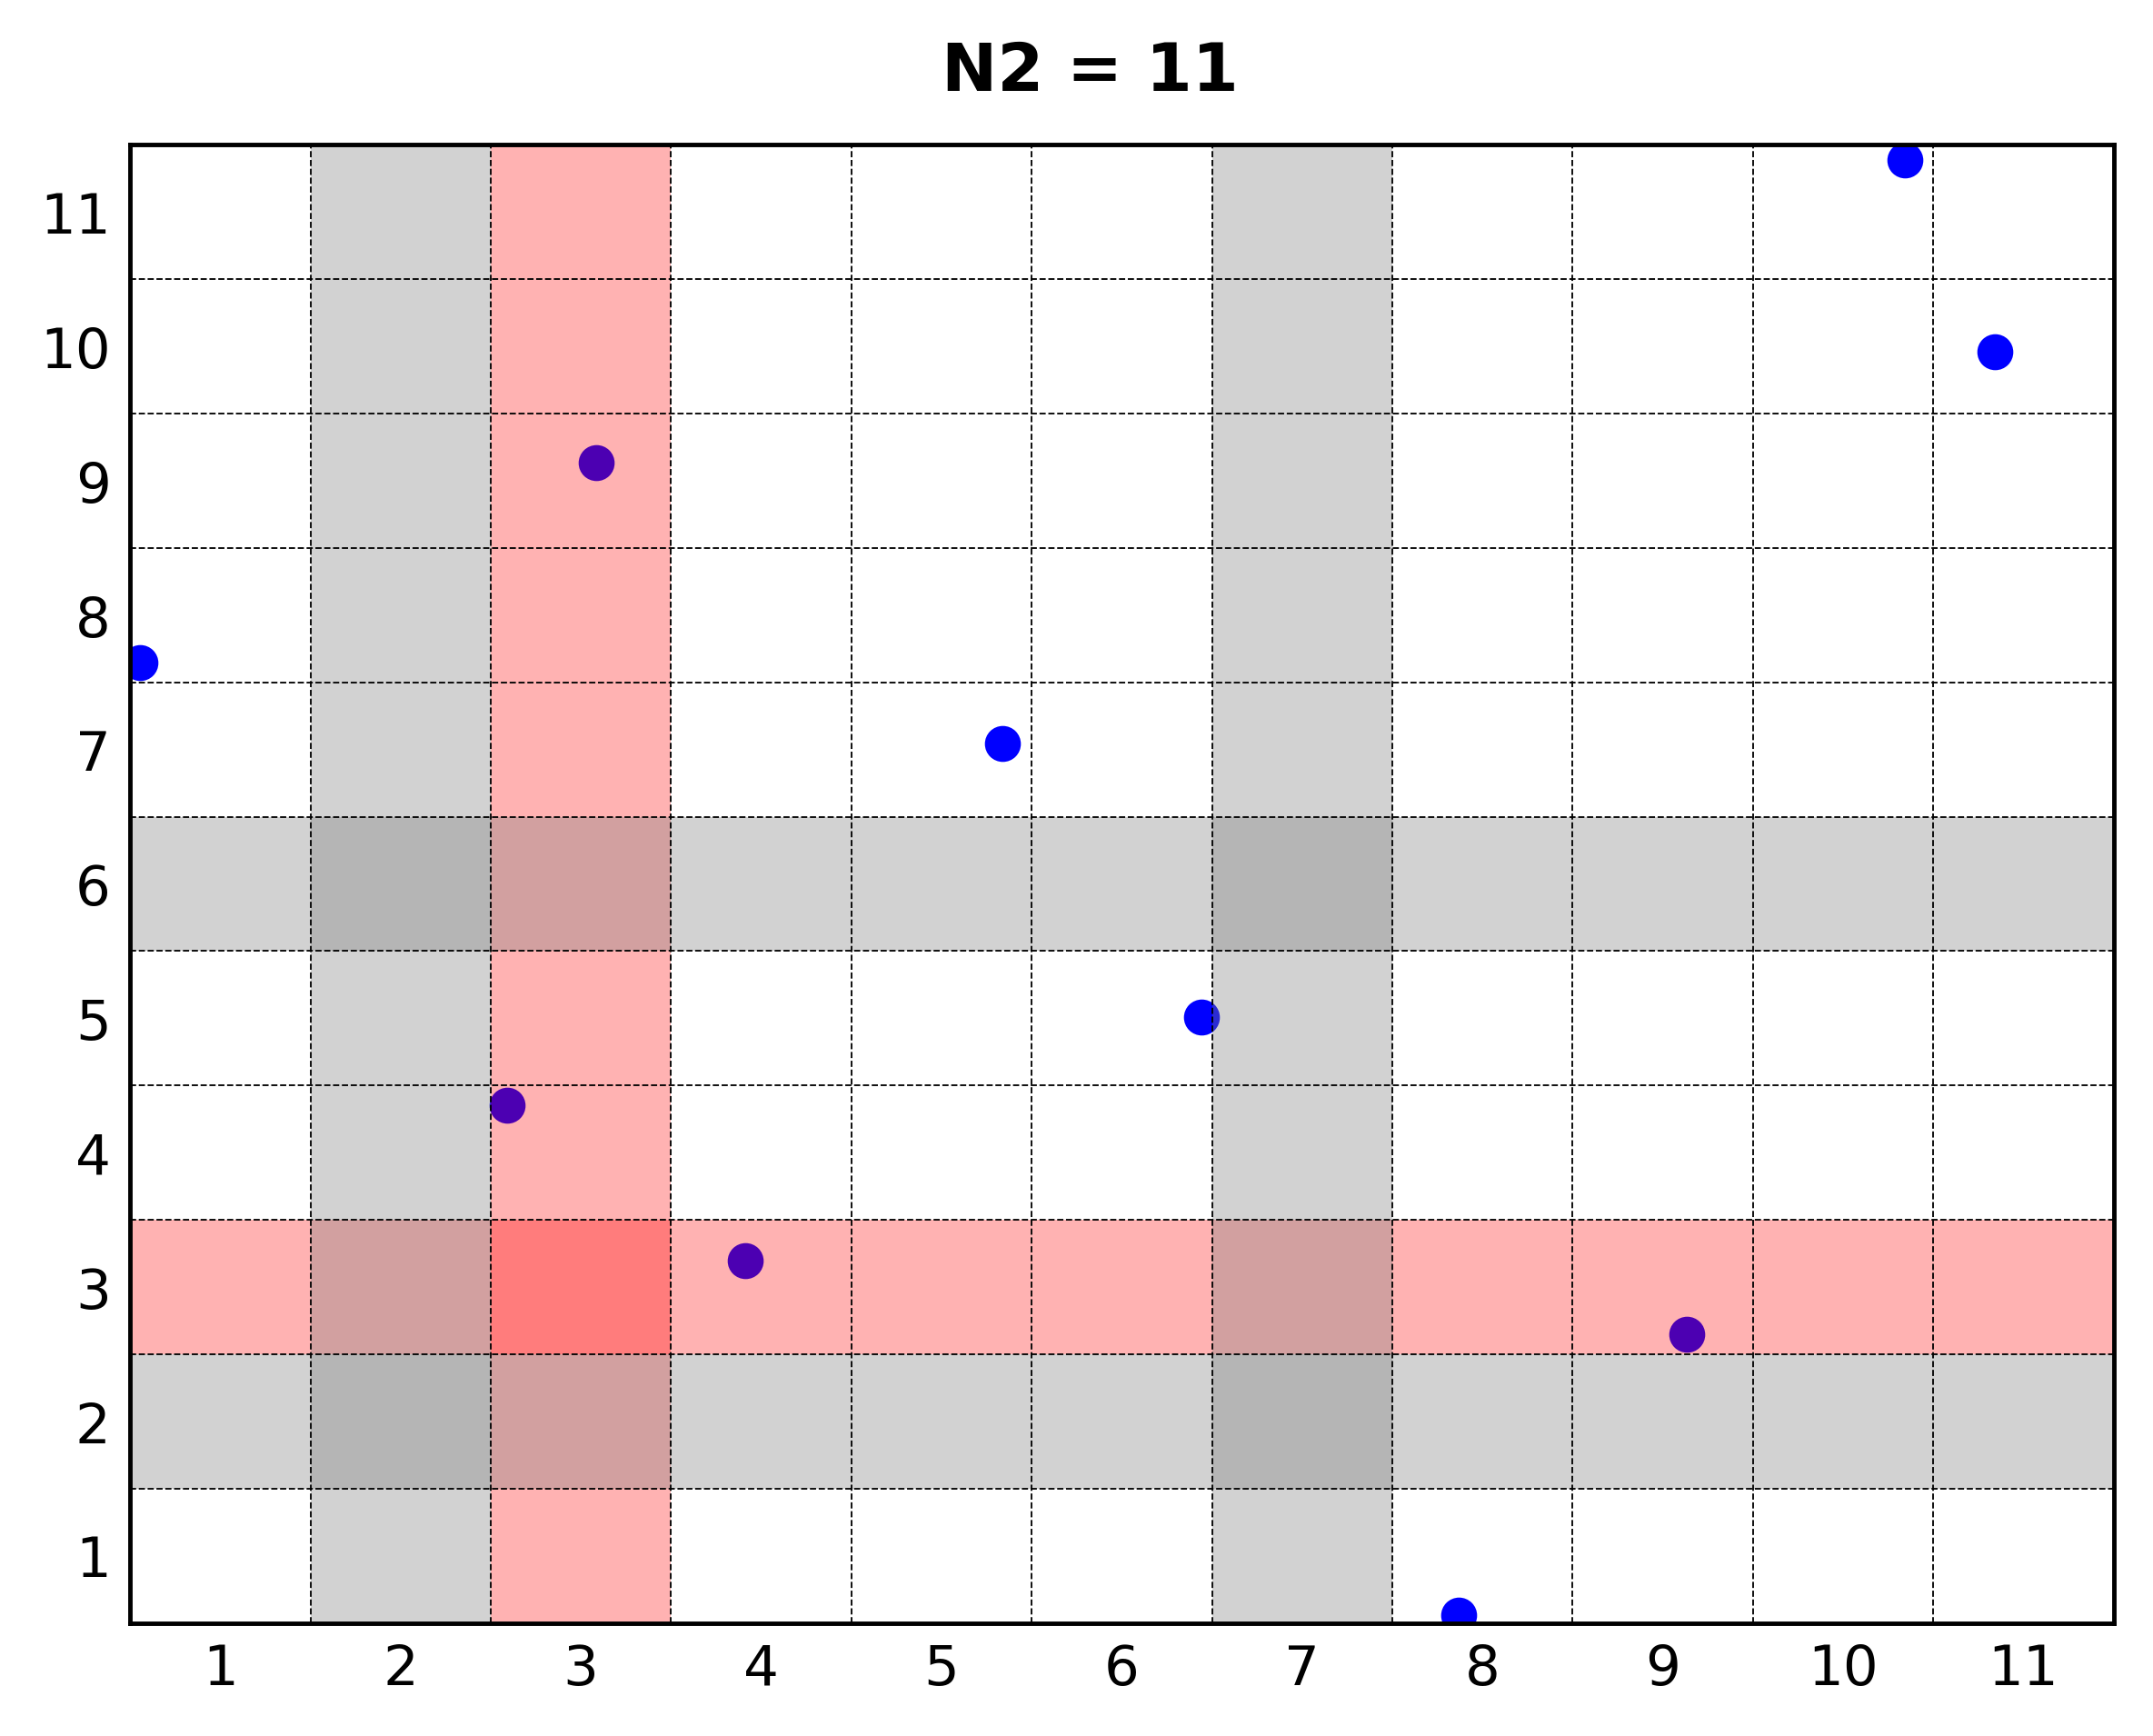
\includegraphics[width=\textwidth]{src/imgs/example_overlaps2.png}
        	\label{fig:example_overlaps2}
        }
    \end{subfigure}
    
    \begin{subfigure}[b]{0.49\textwidth}
        \centering
        \vtop{
        	\vspace{0pt}
        	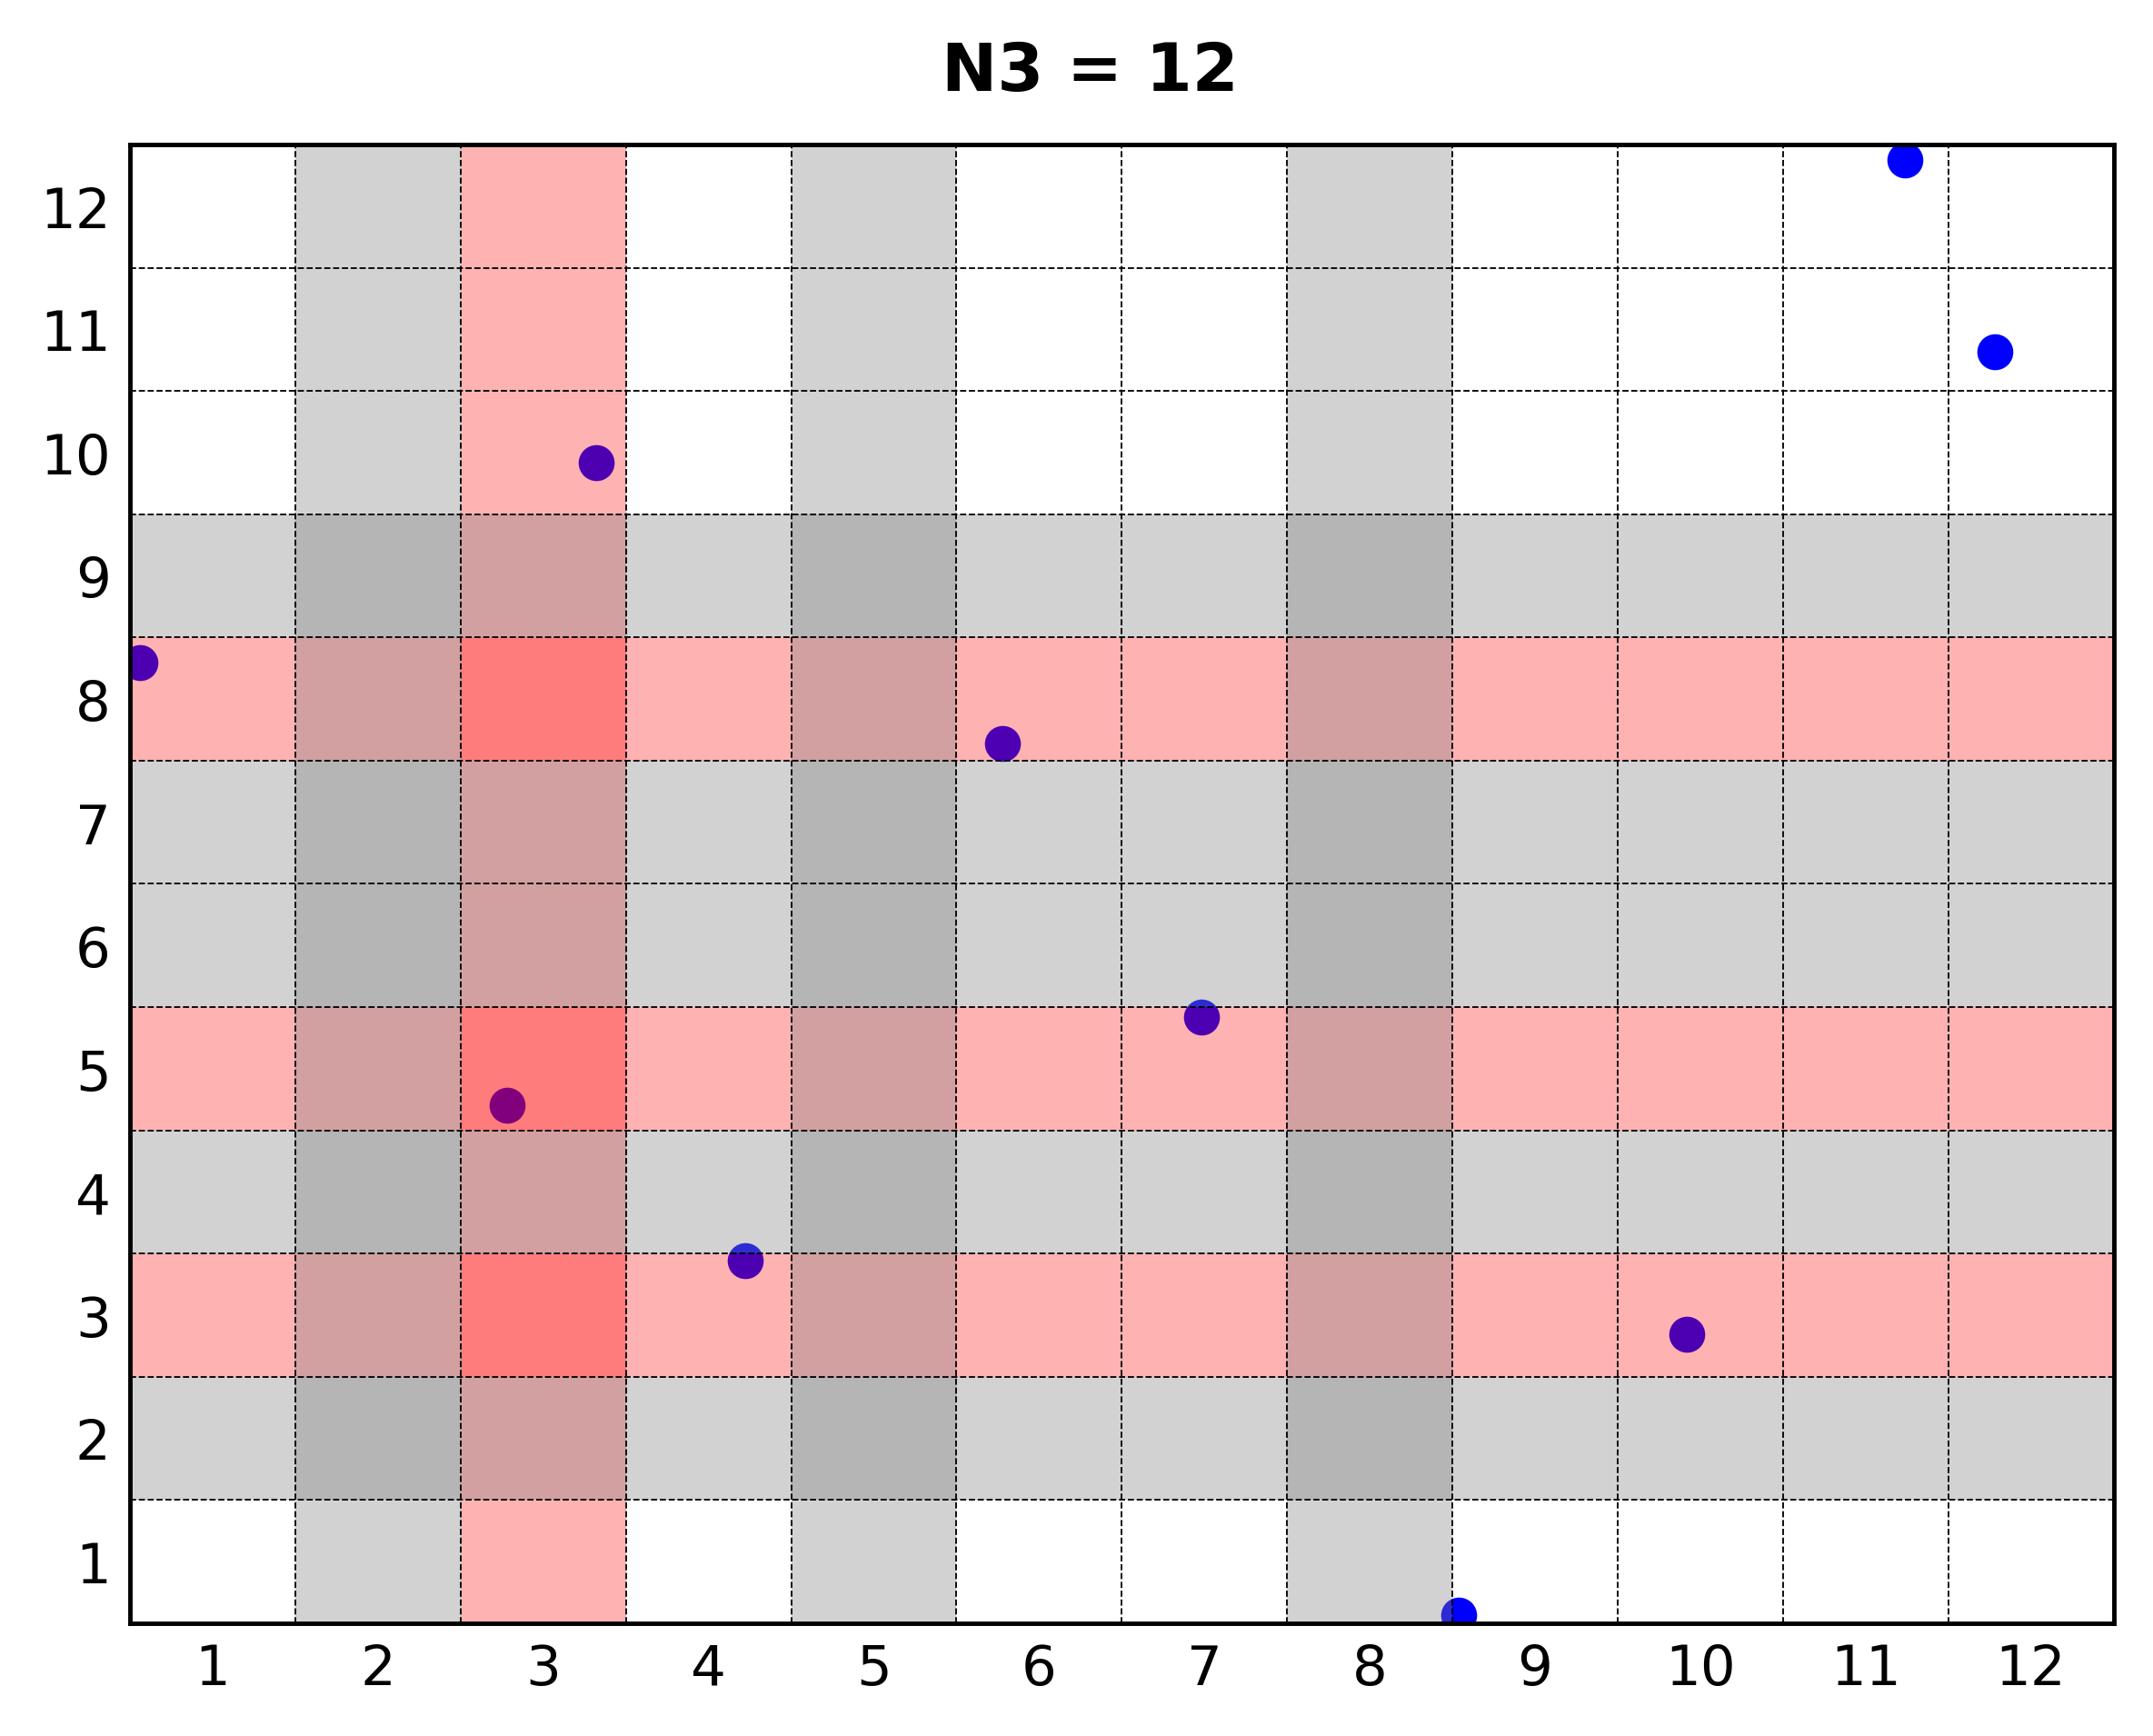
\includegraphics[width=\textwidth]{src/imgs/example_overlaps3.png}
        	\captionsetup{skip=0pt}
        	\midcaption{}
        	\label{fig:example_overlaps3}
        }
    \end{subfigure}
    %\hspace{0.01\textwidth}
    \begin{subfigure}[b]{0.49\textwidth}
        \centering
        \vtop{
        	\vspace{0pt}
        	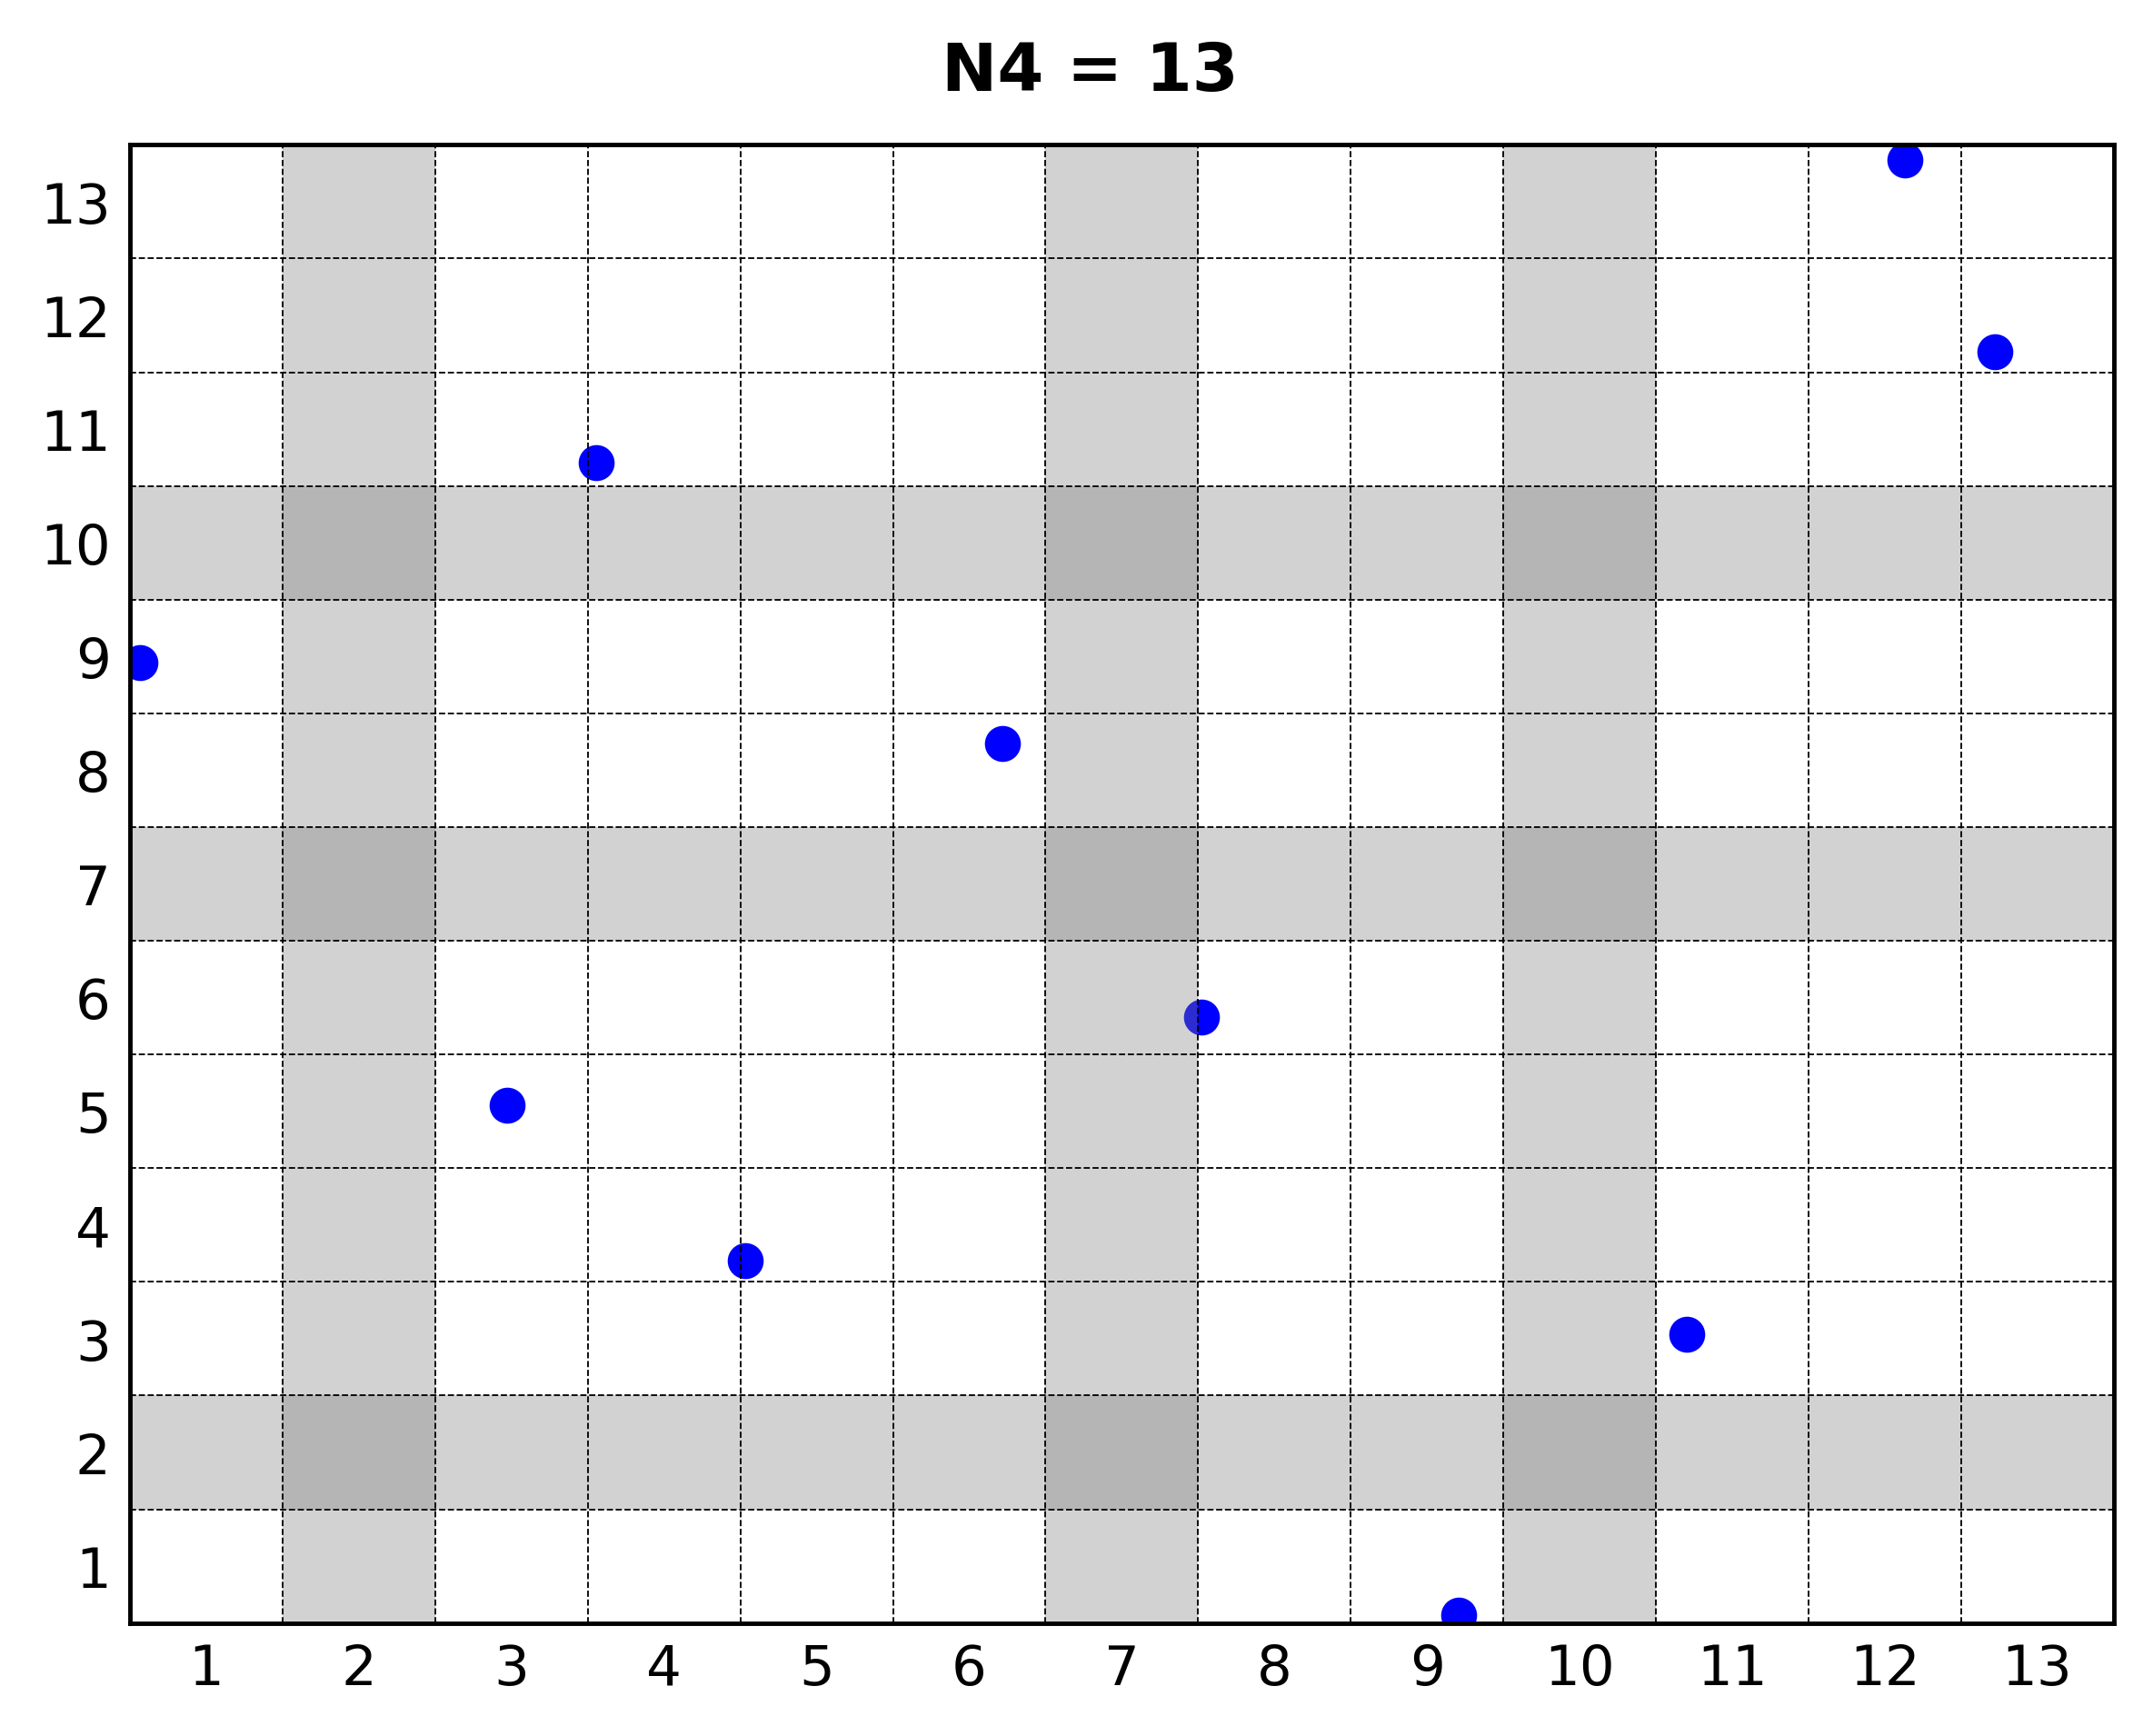
\includegraphics[width=\textwidth]{src/imgs/example_overlaps4.png}
        	\captionsetup{skip=0pt}
        	\midcaption{}
        	\label{fig:example_overlaps4}
        }
    \end{subfigure}
    
    \caption{To demonstrate the behavior of the grid, $S \in LHS(N_1 = 10, P = 2)$ sample set is allocated and projected over the grid as it grows one by one. Rows and columns marked in red indicate the location of overlaps, while light grey-colored rows and columns are vacant. In (a) $N_1 = 10$ LHS samples are displayed over a grid of $N_1$ intervals per axis; (b) shows the first step of the growing grid: two overlaps occur in the horizontal and vertical intervals \#3, two intervals per dimension are vacant one of which derives from the expansion vacancy and the other one is caused by the overlap; (c) samples displayed over $N_3 = N_1 + 2$ grid: on the vertical axis there are 3 overlaps and 2 (from the expansion) + 3 (from the overlaps) vacancies; (d) the grown $N_4 = N_1 + 3$ grid have no collisions, then $S$ is a perfect expansion with $M = 3$ expansion magnitude}
    \label{fig:example_overlaps}
\end{figure}


\subsection{Degree of an Expansion}
\label{subsec:expansion_degree}
A precise heuristic that expresses how near the current expansion is to a perfect expansion, given the desired expansion magnitude $M$ and the beginning state, is necessary for developing a new sample set. Since the metric in \meqref{eq:degree} is no longer sufficient, the variation \textit{expanded degree} has been offered.
The purpose of the \textit{expanded degree} is to convert the sample set $S$ of $N$ elements into an index when the sample set is compared against a $P$-dimensional hypercube grid of $N+M$ intervals per axis - this is where it deviates from \meqref{eq:degree}. Here it follows:

\begin{equation}
\label{eq:expanded_degree}
\mathcal{D}(S, M) := \frac{\sum^P_{j=1}\sum^{N + M}_{q=1} min(\sum^N_{i=1}\indfunc{[\frac{q-1}{N + M}, \frac{q}{N + M})}(S_{ij}), 1)}{P \cdot (N + M)}
\end{equation}

Each $I$ interval contributes to \meqref{eq:expanded_degree} value with a share of:

\begin{equation}
\label{eq:single_contribute_interval}
\mu_I = 
\begin{cases}
\frac{1}{P \cdot (N+M)} \qquad \text{\textit{if any x $\in$ I}}\\
0 \qquad\qquad\;\;\; \text{\textit{otherwise}}
\end{cases}
\end{equation}

which makes \meqref{eq:expanded_degree} a discrete quantity that ranges from $\frac{1}{N+M}$, if every sample of a non-empty set lies in one single interval per axis, to 1, which represents the perfect LHS expansion.

A perfect expansion for $S \in MC(N, P)$ over a $N+M$ space grid of a number $M$ of intervals (per dimension) empty, given that, by definition of LHS, $N$ samples fall in $N$ distinct intervals (per dimension). Then, the only valuable \textbf{$\mu$} shares are given by $N$ intervals while the other $M$ set of intervals are empty. From this statement, we can provide an upper limit for the expanded degree by starting from 1 - the maximum possible index of a perfect LHS sample set - minus the total weight lost during the growing of the grid, which corresponds to the total number of \textit{voids} times \meqref{eq:single_contribute_interval}. The total number of \textit{voids} is equal to $M \cdot P$ because they are evenly spread across each dimension. So, $Z$ is a \textit{perfect expansion} of $S$ with $M$ additional intervals if and only if:

\begin{equation}
\label{eq:upper_limit_perfect_expansion}
gr_{max}(S, M) = 1 - \frac{M}{N+M}
\end{equation}

The \textit{initial set} $S \in MC(N, P)$ plotted over $P$ hypercube of $M+N$ intervals (per dimension) is called \textit{perfect expansion} if and only if $S$ expanded degree \meqref{eq:expanded_degree} is equal to the \textit{upper expanded degree limit} \meqref{eq:upper_limit_perfect_expansion}. \\
As the name may suggest, the perfect expansion is the best possible candidate to produce an optimal stratified sample set, so an LHS, as result of an expansion process described in \cref{subsubsec:general_expansion_case}.


\subsection{The expansion process}
The expansion task was initially handed at the very beginning of  \cref{subsec:multistage_task} as a evolutionary process which augments the $S$ starting sample set to a next-stage state with increased number of elements $M$, placed as better as it can to maximize criteria. However, we show in \cref{subsec:expansion_degree} that an expansion may demote the stratification of the resultant expanded set $Z$, which can be measured with the metric \meqref{eq:expanded_degree}. 
In this section the authors propose how to place the new samples to achieve maximum "LHS-ness" over any $M$ expansion magnitude needed and introduce its potentialities for future researches - see more in \cref{sec:conclusions}.

In first place, the proposal is delivered by studying the basic case of a perfect expansion in \cref{subsubsec:perfect_expansion_case}, then extend to the general case with any non-perfect expansion outcome.

\subsubsection{State case - Perfect Expansion}
\label{subsubsec:perfect_expansion_case}
An initial instanced sample set $S$ of $N$ elements can be perfect expanded if and only if $S$ after the $M$-th growing step of the $P$-hypercube grid has the maximum degree (\meqref{eq:upper_limit_perfect_expansion}). Furthermore, \mfigref{fig:example_overlaps4} well depicts what the experimenters would expect before setting down an expansion set $E$. We notice the best candidate extent is likely the empty intervals (in light grey) because they do not interfere with other well-formed intervals. It is also imperative that the new samples do not overlap onto each other over the vacant space (\textit{vacancies} or \textit{voids}, as we previously called them).

First of all, it's necessary to trace each void's index. Here it comes into use again the permuted index matrix, previously used in \cref{subsec:how_to_lhs} to scatter the samples across the hyper-parameter space. The matrix of voids $P \times M$ is composed by the row vectors: 

\begin{equation}
\label{eq:voids_matrix}
\textbf{V}_j = \bigg( q : \nexists\; x \in S_{ij} \; s.t. \; x \in \Big[\frac{q-1}{N+M}, \frac{q}{N+M}\Big) \bigg) \quad, \quad \forall j = 1...P
\end{equation}

which should be element-wise permuted along each row to prevent \mfigref{fig:diagonal_poor_design} diagonalized situation.
Then, the expansion set $E$ collects all the newly generated samples which are a distribution likewise \meqref{eq:rand_variable_Sij} but using $V_{ji}$. 

In the end, the initial $S$ set is concatenated with expansion set $E$, originated from the voids of the $N+M$ growing grid, in a perfect expansion, that guarantees the fulfilling of maximum stratification (degree = 1). 

A perfect expansion is a intuitively rare event: each sample has to avoid overlaps. This could eventually happen if two sample projections are spaced more than $\frac{1}{N+M}$ apart (new size of the intervals), But if they are closer, another condition has to be fulfilled: for any $M$ close enough to $N$, a \textit{critical span} exists across the \textit{i-th frontier} (see right after \meqref{eq:interval_index} for definition) - which shares its boundary with the next interval. The critical span is the intersection area between two neighbor samples intervals and the eventual interval raised across them (\mfigref{fig:critical_span2}). Given that LHS is not supposed to consider further additional points, it might happen that samples are placed in critical areas (after a $M$ growing step). An example of how can a couple of collapsing samples can occur is shown in \mfigref{fig:critical_span}. In the example, the first sample (in \mfigref{fig:critical_span2}) has been generated in the critical area that is the intersection between \textit{$\sim$2} and \#1 original interval. On its hand, the second sample lies upon the same critical area between \textit{$\sim$2} and \#2 original subspace. Hence, in the example the two samples are overlapped.

\begin{figure}[h]
    \centering
    \begin{subfigure}[b]{0.45\textwidth}
        \centering
        \vtop{
        	\vspace{0pt}
        	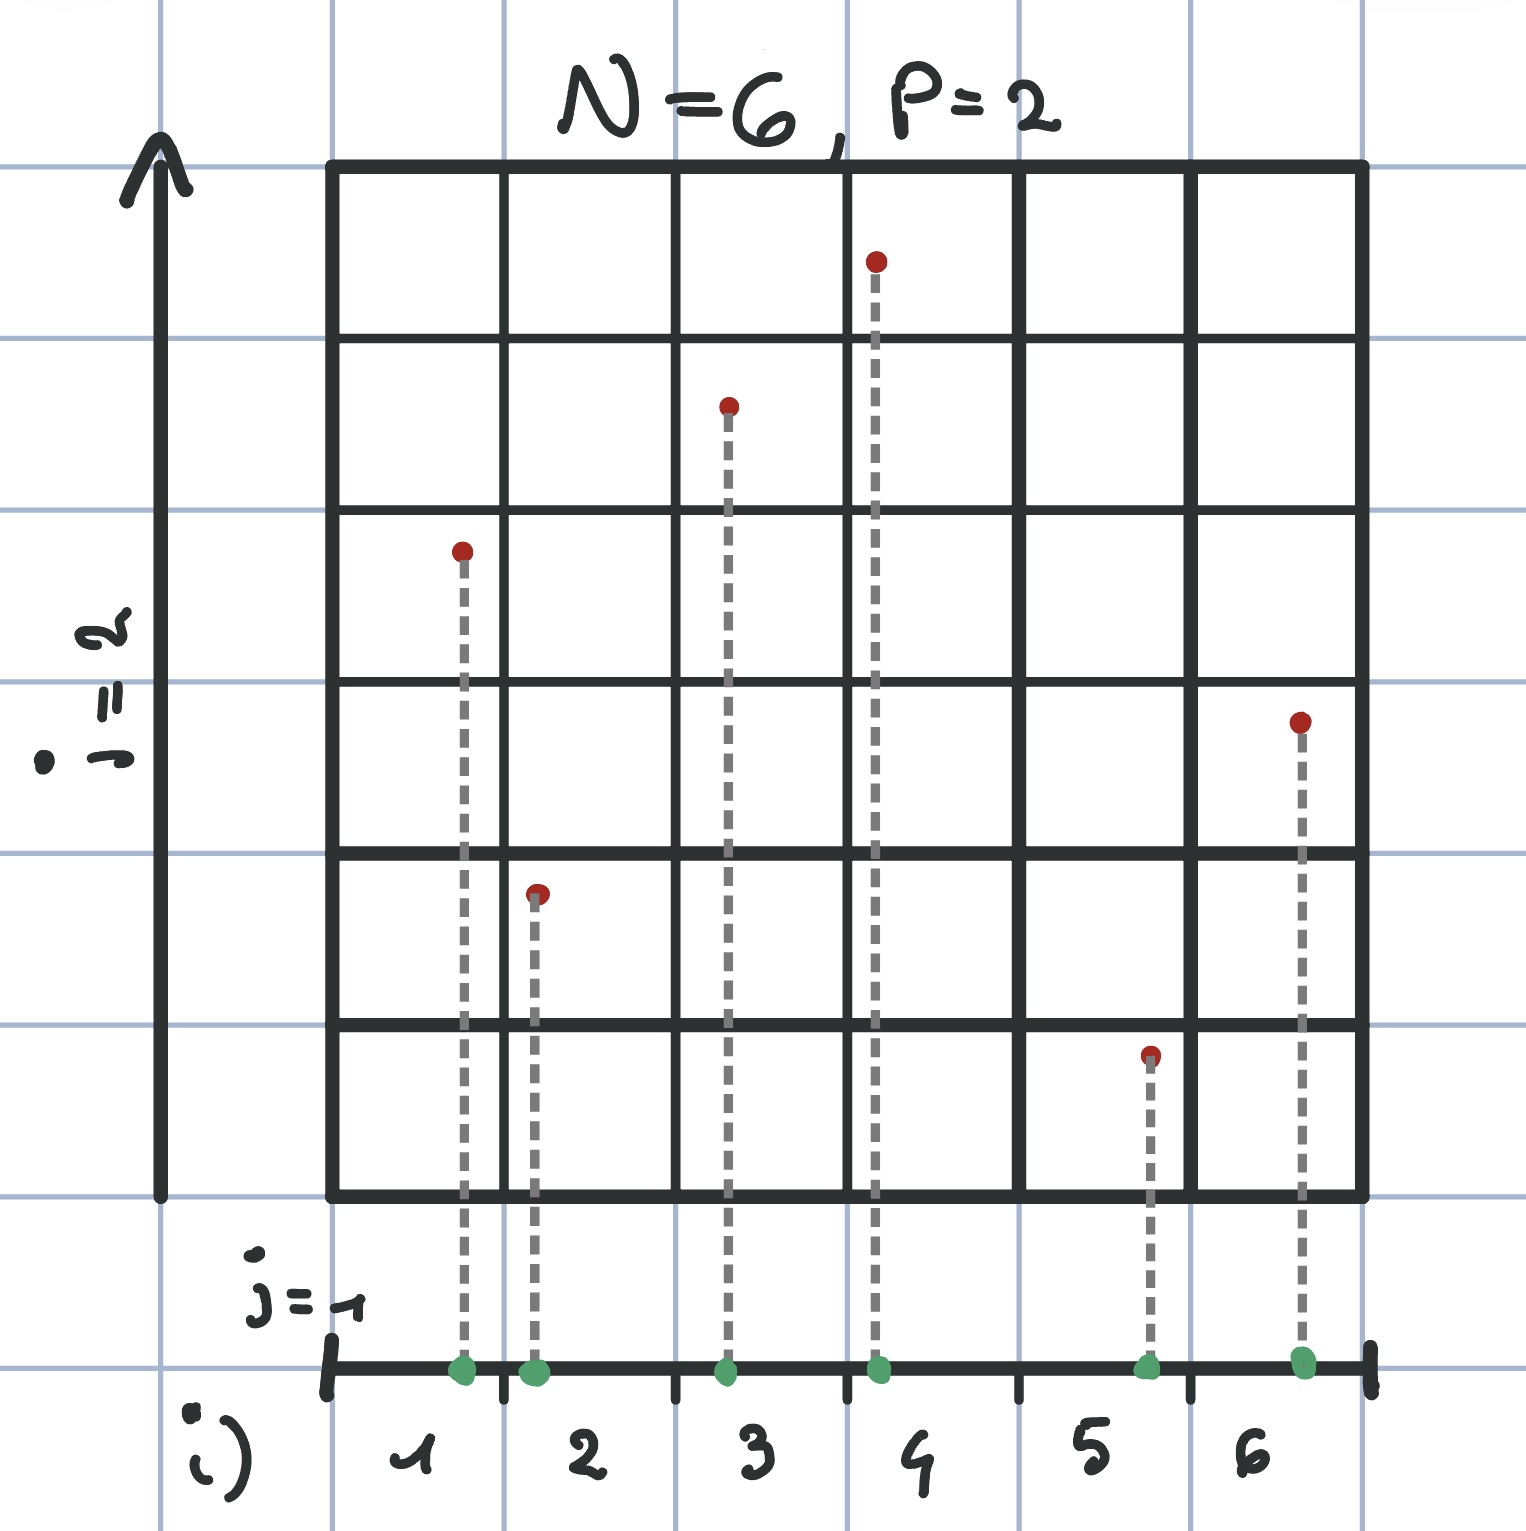
\includegraphics[width=\textwidth]{src/imgs/critical_span_init.jpg}
        	\caption{An LHS of $N = 6$ samples expanded for $M = 2$. on the horizontal axis are projected the horizontal component of all samples. [SKETCH - ne farò in digitale di migliori]}
        	\label{fig:critical_span1}
        }
    \end{subfigure}
    \hspace{0.05\textwidth}
    \begin{subfigure}[b]{0.45\textwidth}
        \centering
        \vtop{
        	\vspace{0pt}
        	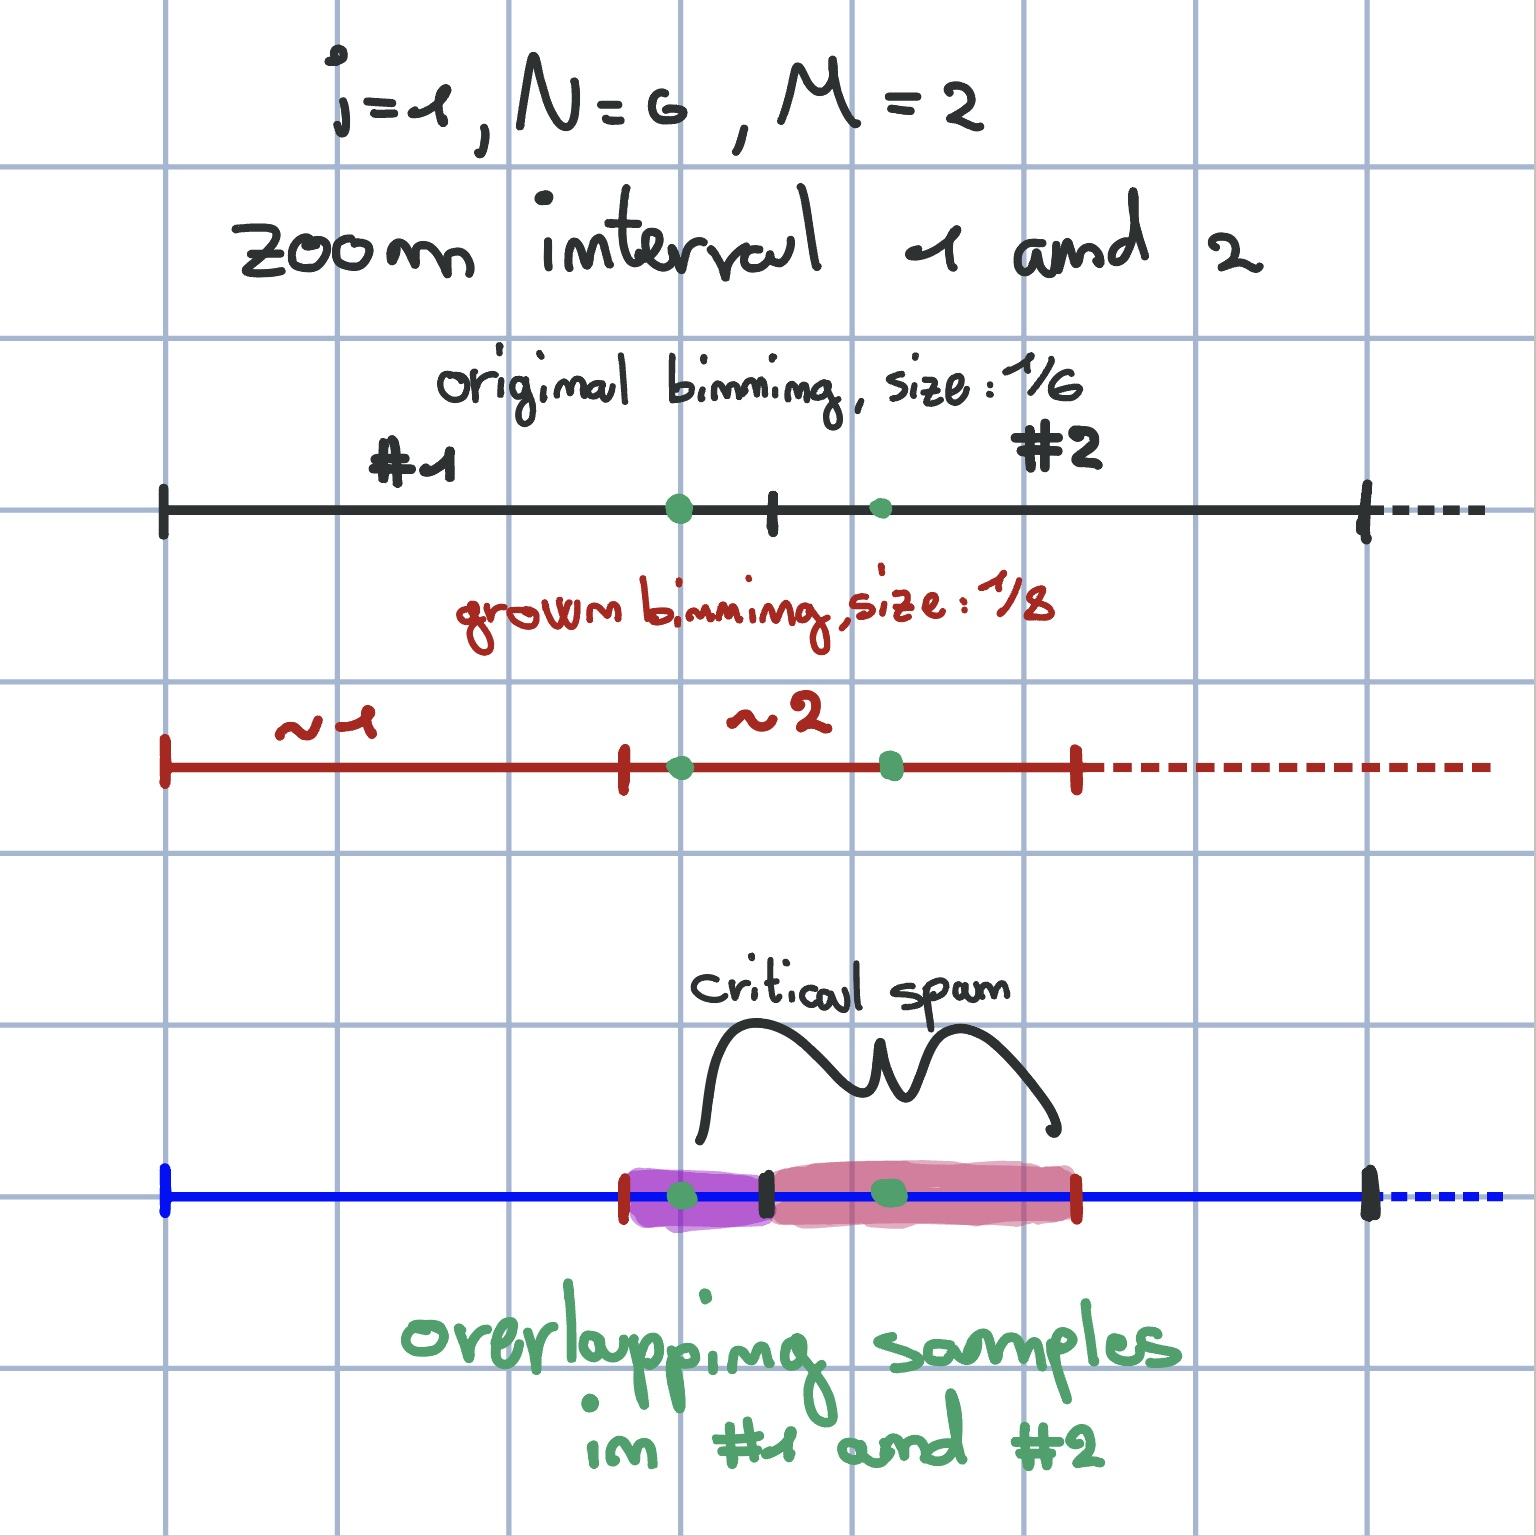
\includegraphics[width=\textwidth]{src/imgs/critical_span_zoom.jpg}
        	\caption{Zooming in \#1 and \#2 interval, it's show how both shares a critical area (on the bottom) whereof each one may have been distributed in it. [SKETCH - ne farò in digitale di migliori]}
        	\label{fig:critical_span2}
        }
    \end{subfigure}
    \midcaption{ }
    \label{fig:critical_span}
\end{figure}
 
The number and displacement of overlaps and vacancies are pretty hard to predict: they are strongly correlated to the \meqref{eq:Sij_def} sample random distribution. However, we experimentally observed that some expansions are peculiar: exactly all expansions with multiples of $N$ are always perfect. That's because critical spans - again, that are given by the intersection of the specific new intervals that cross the old frontiers with the previous intervals - are always void. Take \mfigref{fig:critical_span2} but with grown binning size equals to $\frac{1}{12}$ instead of $\frac{1}{8}$ (so, with $N = 6$ then $M = 12$): new intervals divide perfectly the old ones, without ever crossing any frontier. This concept is properly explained in \mappendixref{appendix:N_multiples}. Explicitly:

\begin{equation}
\label{eq:known_perfect_expansions}
\forall K \in \mathbb{N}^+ \;\; : \;\; S \in LHS(N, P) \Rightarrow \mathcal{D}(S, K \cdot N) = gr_{max}
\end{equation}

[I'm not exactly sure if it should be $\Rightarrow$ or $\Leftrightarrow$]

\subsubsection{State case - General Expansion}
\label{subsubsec:general_expansion_case}
During the upscale of $S$ from $N$ to $N+M$ number of elements, it comes along with a variable number of overlaps on j-th axis $O_j$.
In \cref{subsec:expansion_degree} the authors stress the relation between tuples $\textbf{V}_j$, $M$, and the amount of collisions $O_j$ on each j-th dimension. Specifically:
\begin{equation}
\label{eq:vjojm}	% nome norvegese di alto rango
\parallel \textbf{V}_j \parallel = O_j + M
\end{equation}
whereof the overlaps count equals to zero, the expansion has been perfect (see \cref{subsec:multistage_task}). In a general case of expansion, the overlaps amount is most likely not equal to zero in some dimensions.

The case study implies that the creation of the expansion set i$E$ is not trivial anymore because of the irregularity of the vacancies set. By referring to \meqref{eq:vjojm}, unlike what was stated before, $V$ would probably be no matrix at all but, instead, a set of heterogeneous tuples. If $V$ components was homogeneous, it would have been a inherited matrix. The number of $\textbf{V}_j$ interval indexes would likely be more than $M$ sample's projections to commit. The expansion algorithm has to pick up a reasonable subset of $M$ void entries, and thus to discard an amount of intervals equal to the number of overlaps $O_j$. Therefore, given the sub-hyperspace settled by the joined selected voids, in order to plot an $M$ amount of new samples, it will pick up an $P \times M$ submatrix (that mimics \meqref{eq:voids_matrix}) of $V$ set. The submatrix should be handled being aware that it would effect the samples layout which may better improve another coherent criteria chosen (such as low-discrepancy or Maximin space-filling).\\
The selection process of vacancies from an irregular $V$ voids set is described by a function $\sigma: N \times P, \; M \rightarrow P \times M$, namely \textit{perfectify} or \textit{vacancy reduction} (for the matter of giving names to anything). \\ 
In this section, $\sigma$ reduce function trivially picks up $M$ intervals randomly per dimension and build up a permuted \meqref{eq:voids_matrix} vacancies matrix, which will be plugged into \meqref{eq:Sij_def} to produce an expansion set. 

In other words, $\sigma$ criterion extracts from each j-th axis of the vacancies set $\textbf{V}_j$ a fixed $M$ number of elements which are going to compose the sub-hyperspace where $M$ samples will be placed using at least the non-overlapping property. The function $\sigma$ discards $O_j$ number of intervals (\meqref{eq:vjojm}), then creating an amount of voids of the same quantity. Hence, the number of overlaps $O_j$ determines the number of void intervals after the expansion is consumed.

In this paper, the term \textit{quasi-LHS} refers to a non full-degreed in-th stage of expansion descended from a proper LHS.

\begin{figure}[]
    \centering
    \begin{subfigure}[b]{0.45\textwidth}
        \centering
        \vtop{
        	\vspace{0pt}
        	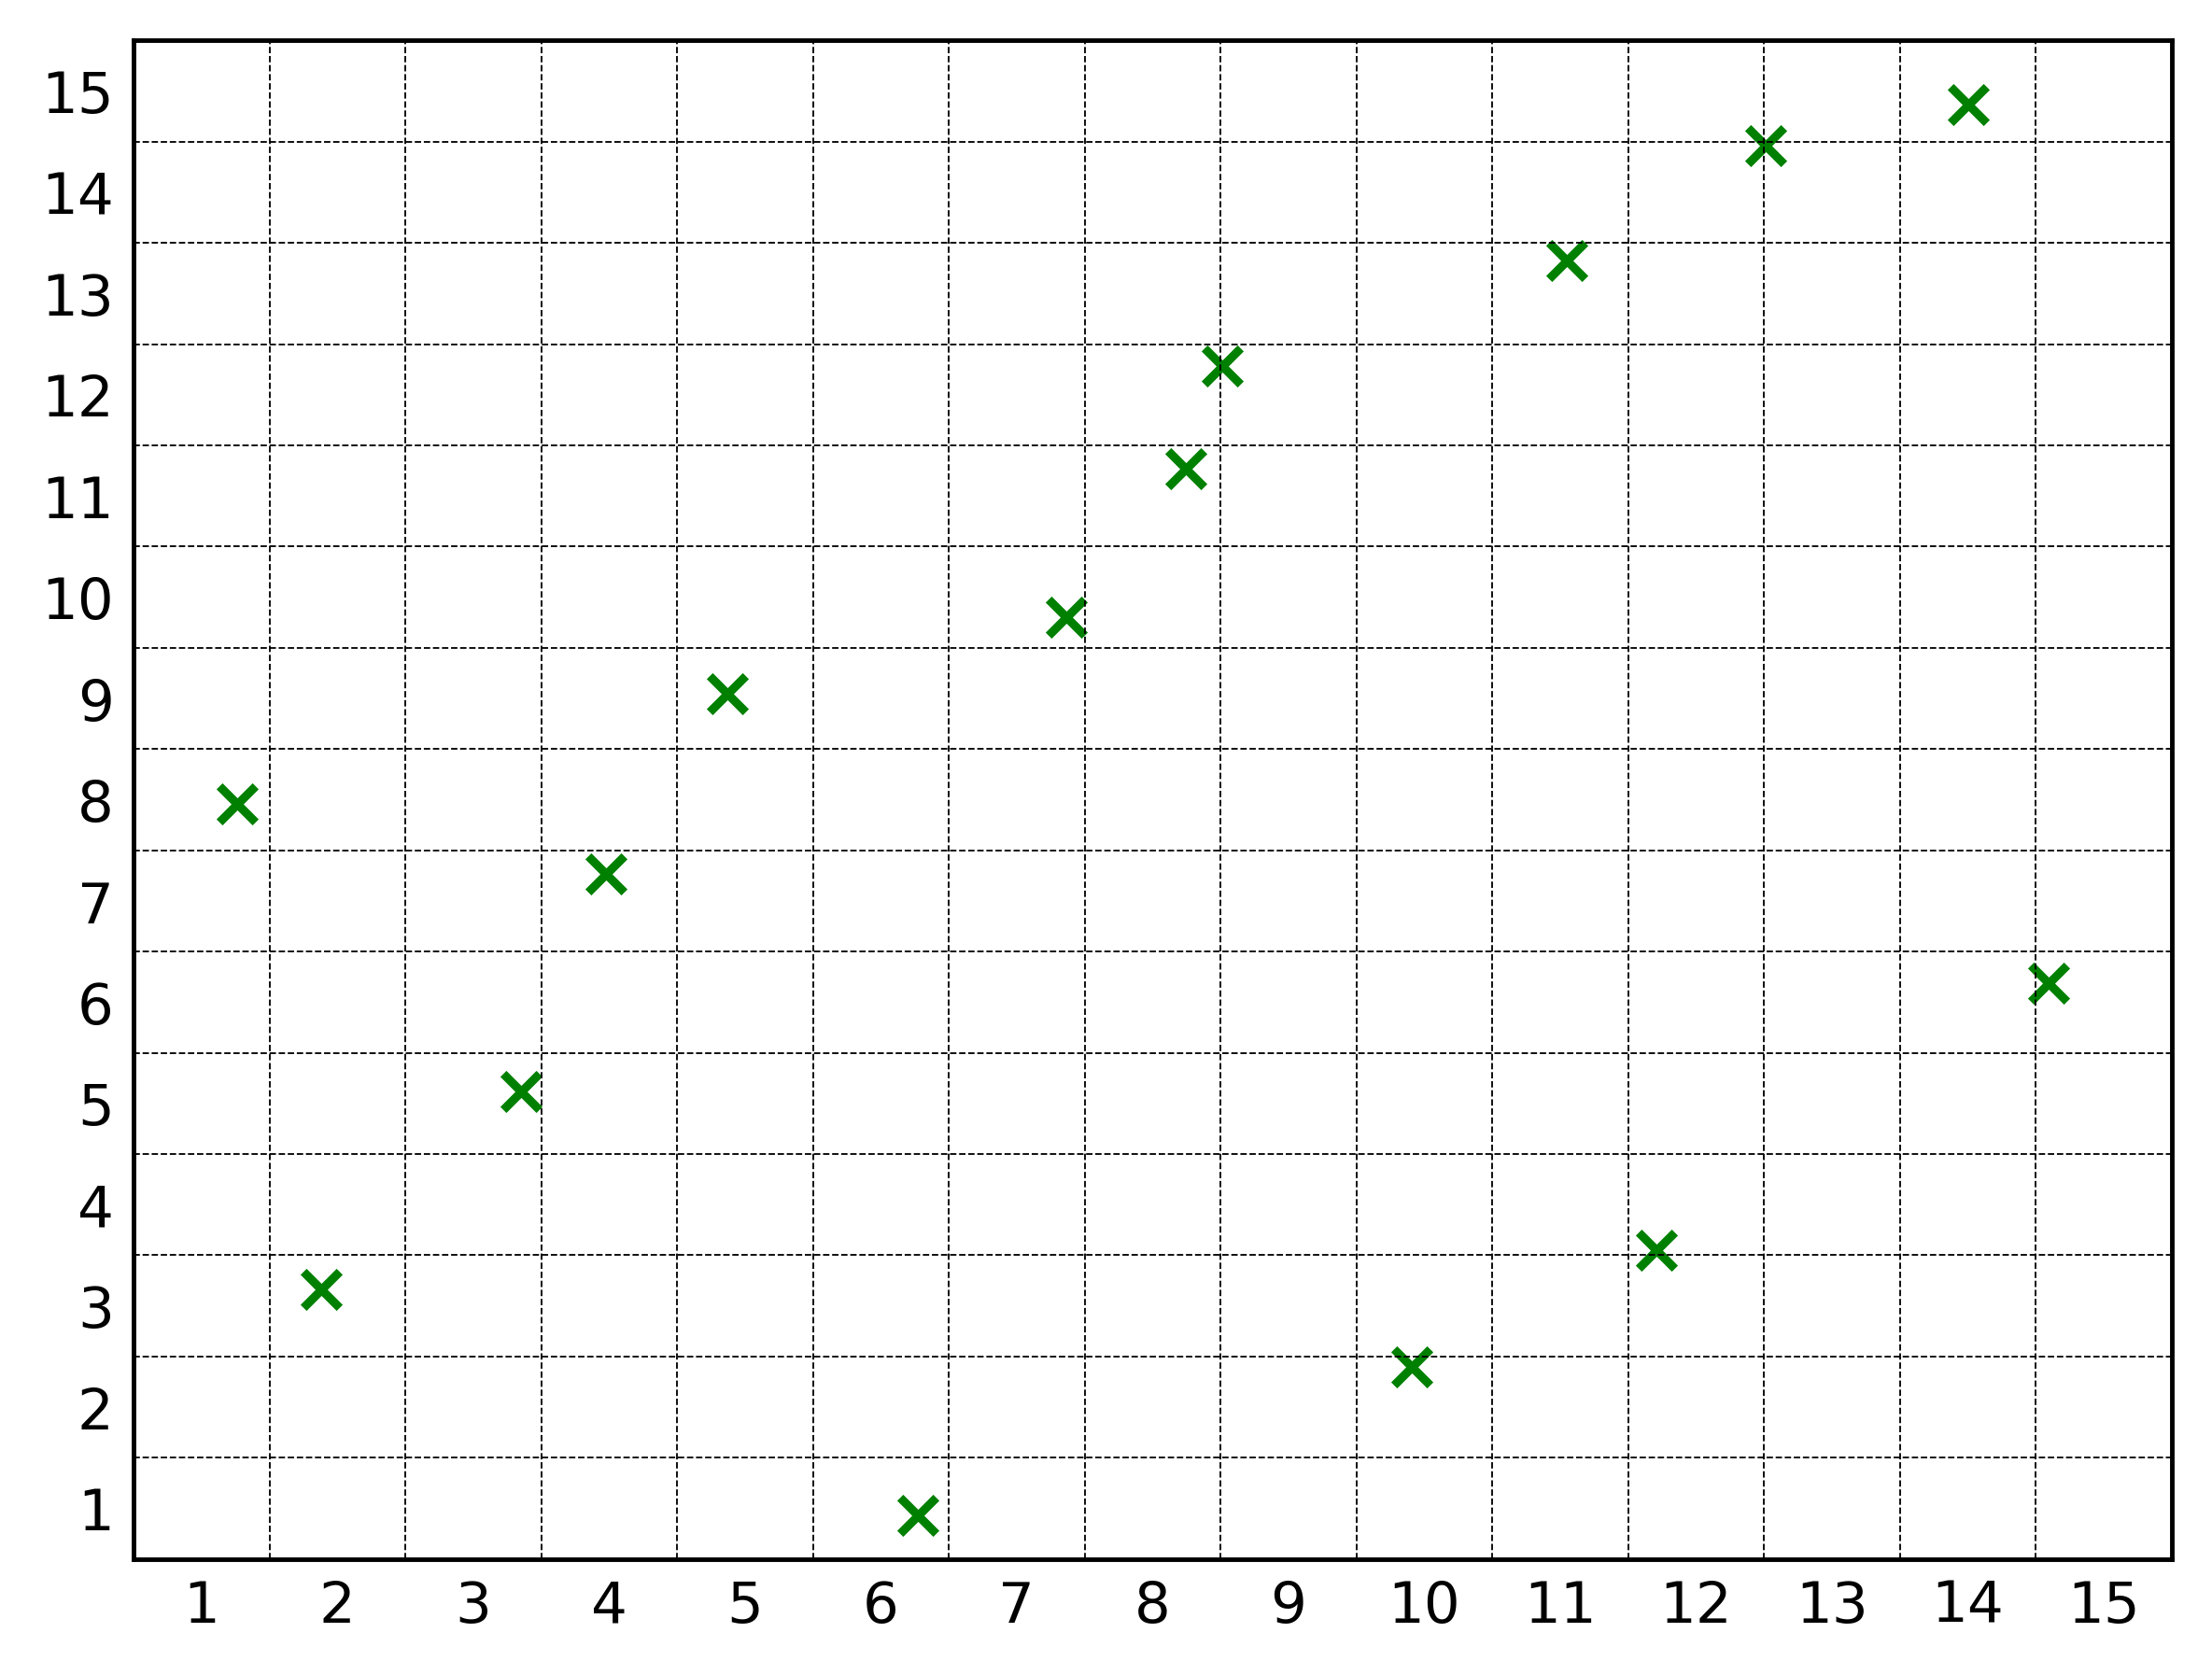
\includegraphics[width=\textwidth]{src/imgs/algo1.png}
        	\captionsetup{skip=0pt}
        	\caption{First-stage LHS of $N = 15$ samples in $P = 2$ generated with scipy's qmc library.}
        	\label{fig:algo1}
        }
    \end{subfigure}
    \hspace{0.05\textwidth}
    \begin{subfigure}[b]{0.45\textwidth}
        \centering
        \vtop{
        	\vspace{0pt}
        	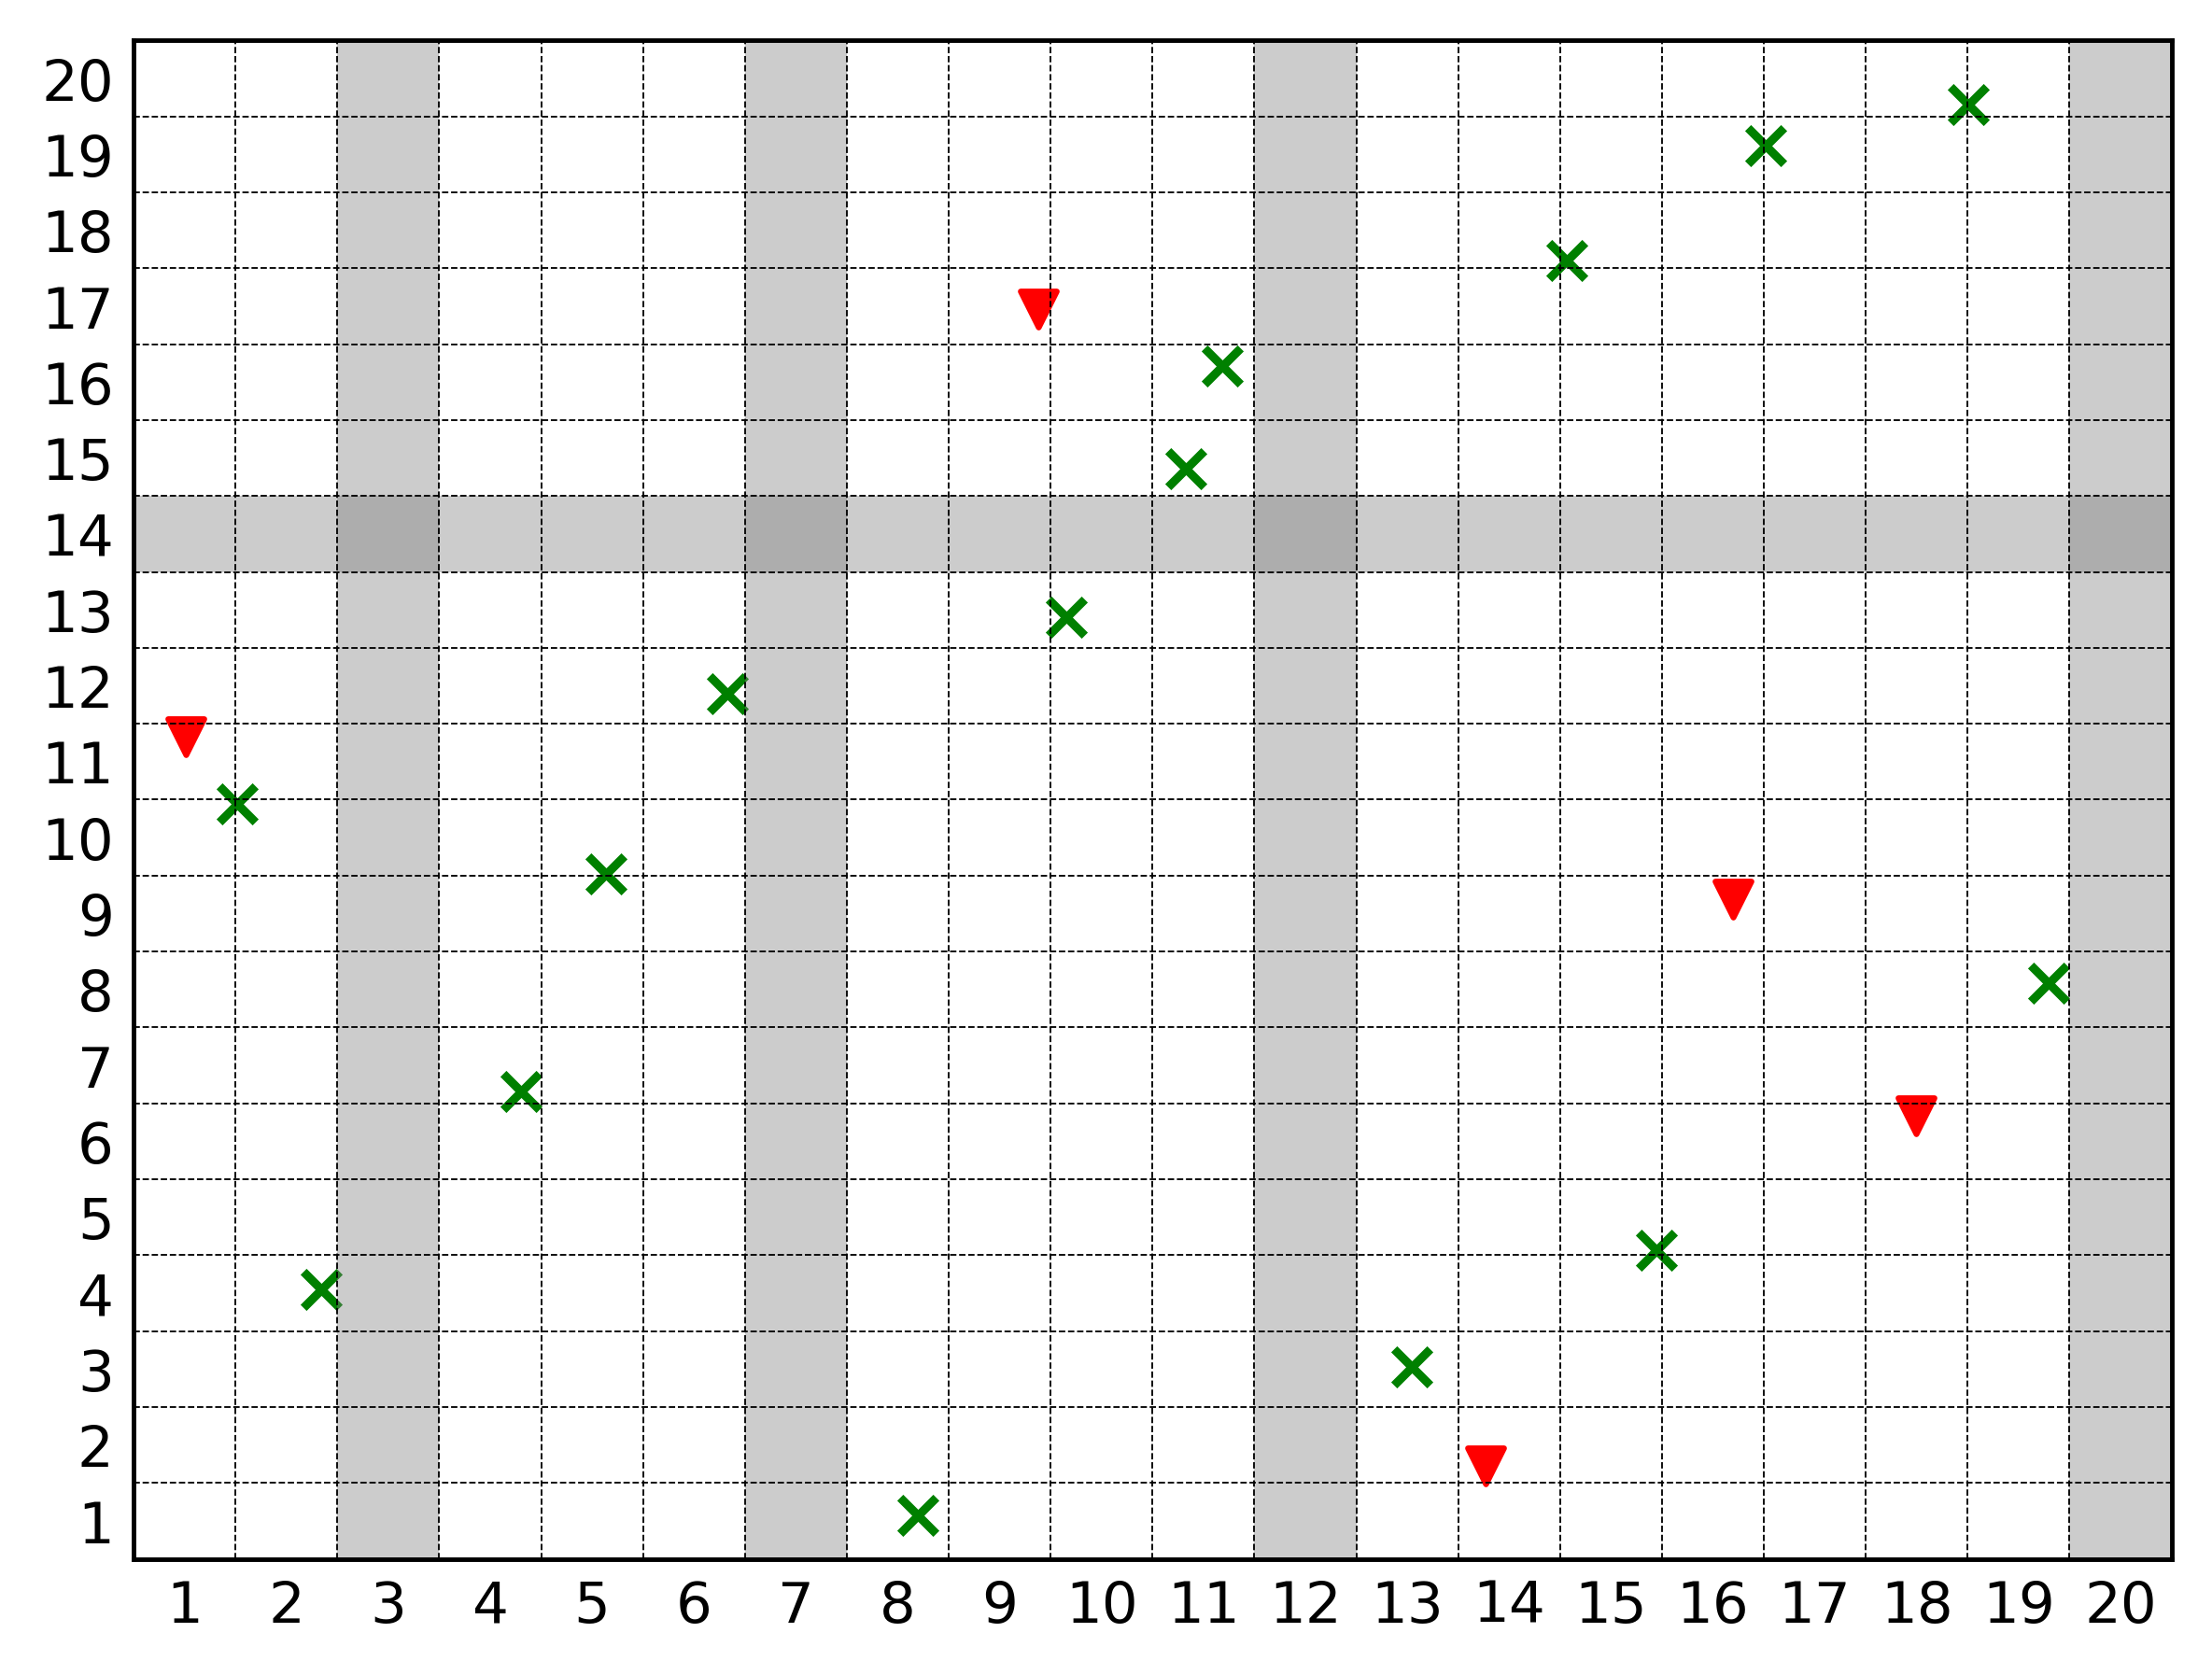
\includegraphics[width=\textwidth]{src/imgs/algo4.png}
        	\captionsetup{skip=0pt}
        	\caption{Expansion of (a)'s LHS with \cref{subsubsec:algorithm} eLHS algorithm given $M = 5$ new samples. Note that the light grey marked intervals are empty and, according to \cref{subsubsec:general_expansion_case}, they are related with the overlaps distribution in (c)}
        	\label{fig:algo2}
        }
    \end{subfigure}
    \captionsetup{justification=centering}
    \caption*{Above is shown a two-staged quasi-LHS. (a) is the first original LHS and (b) is next stage expansion of it.}
    
    \begin{subfigure}[b]{0.45\textwidth}
        \centering
        \vtop{
        	\vspace{0pt}
        	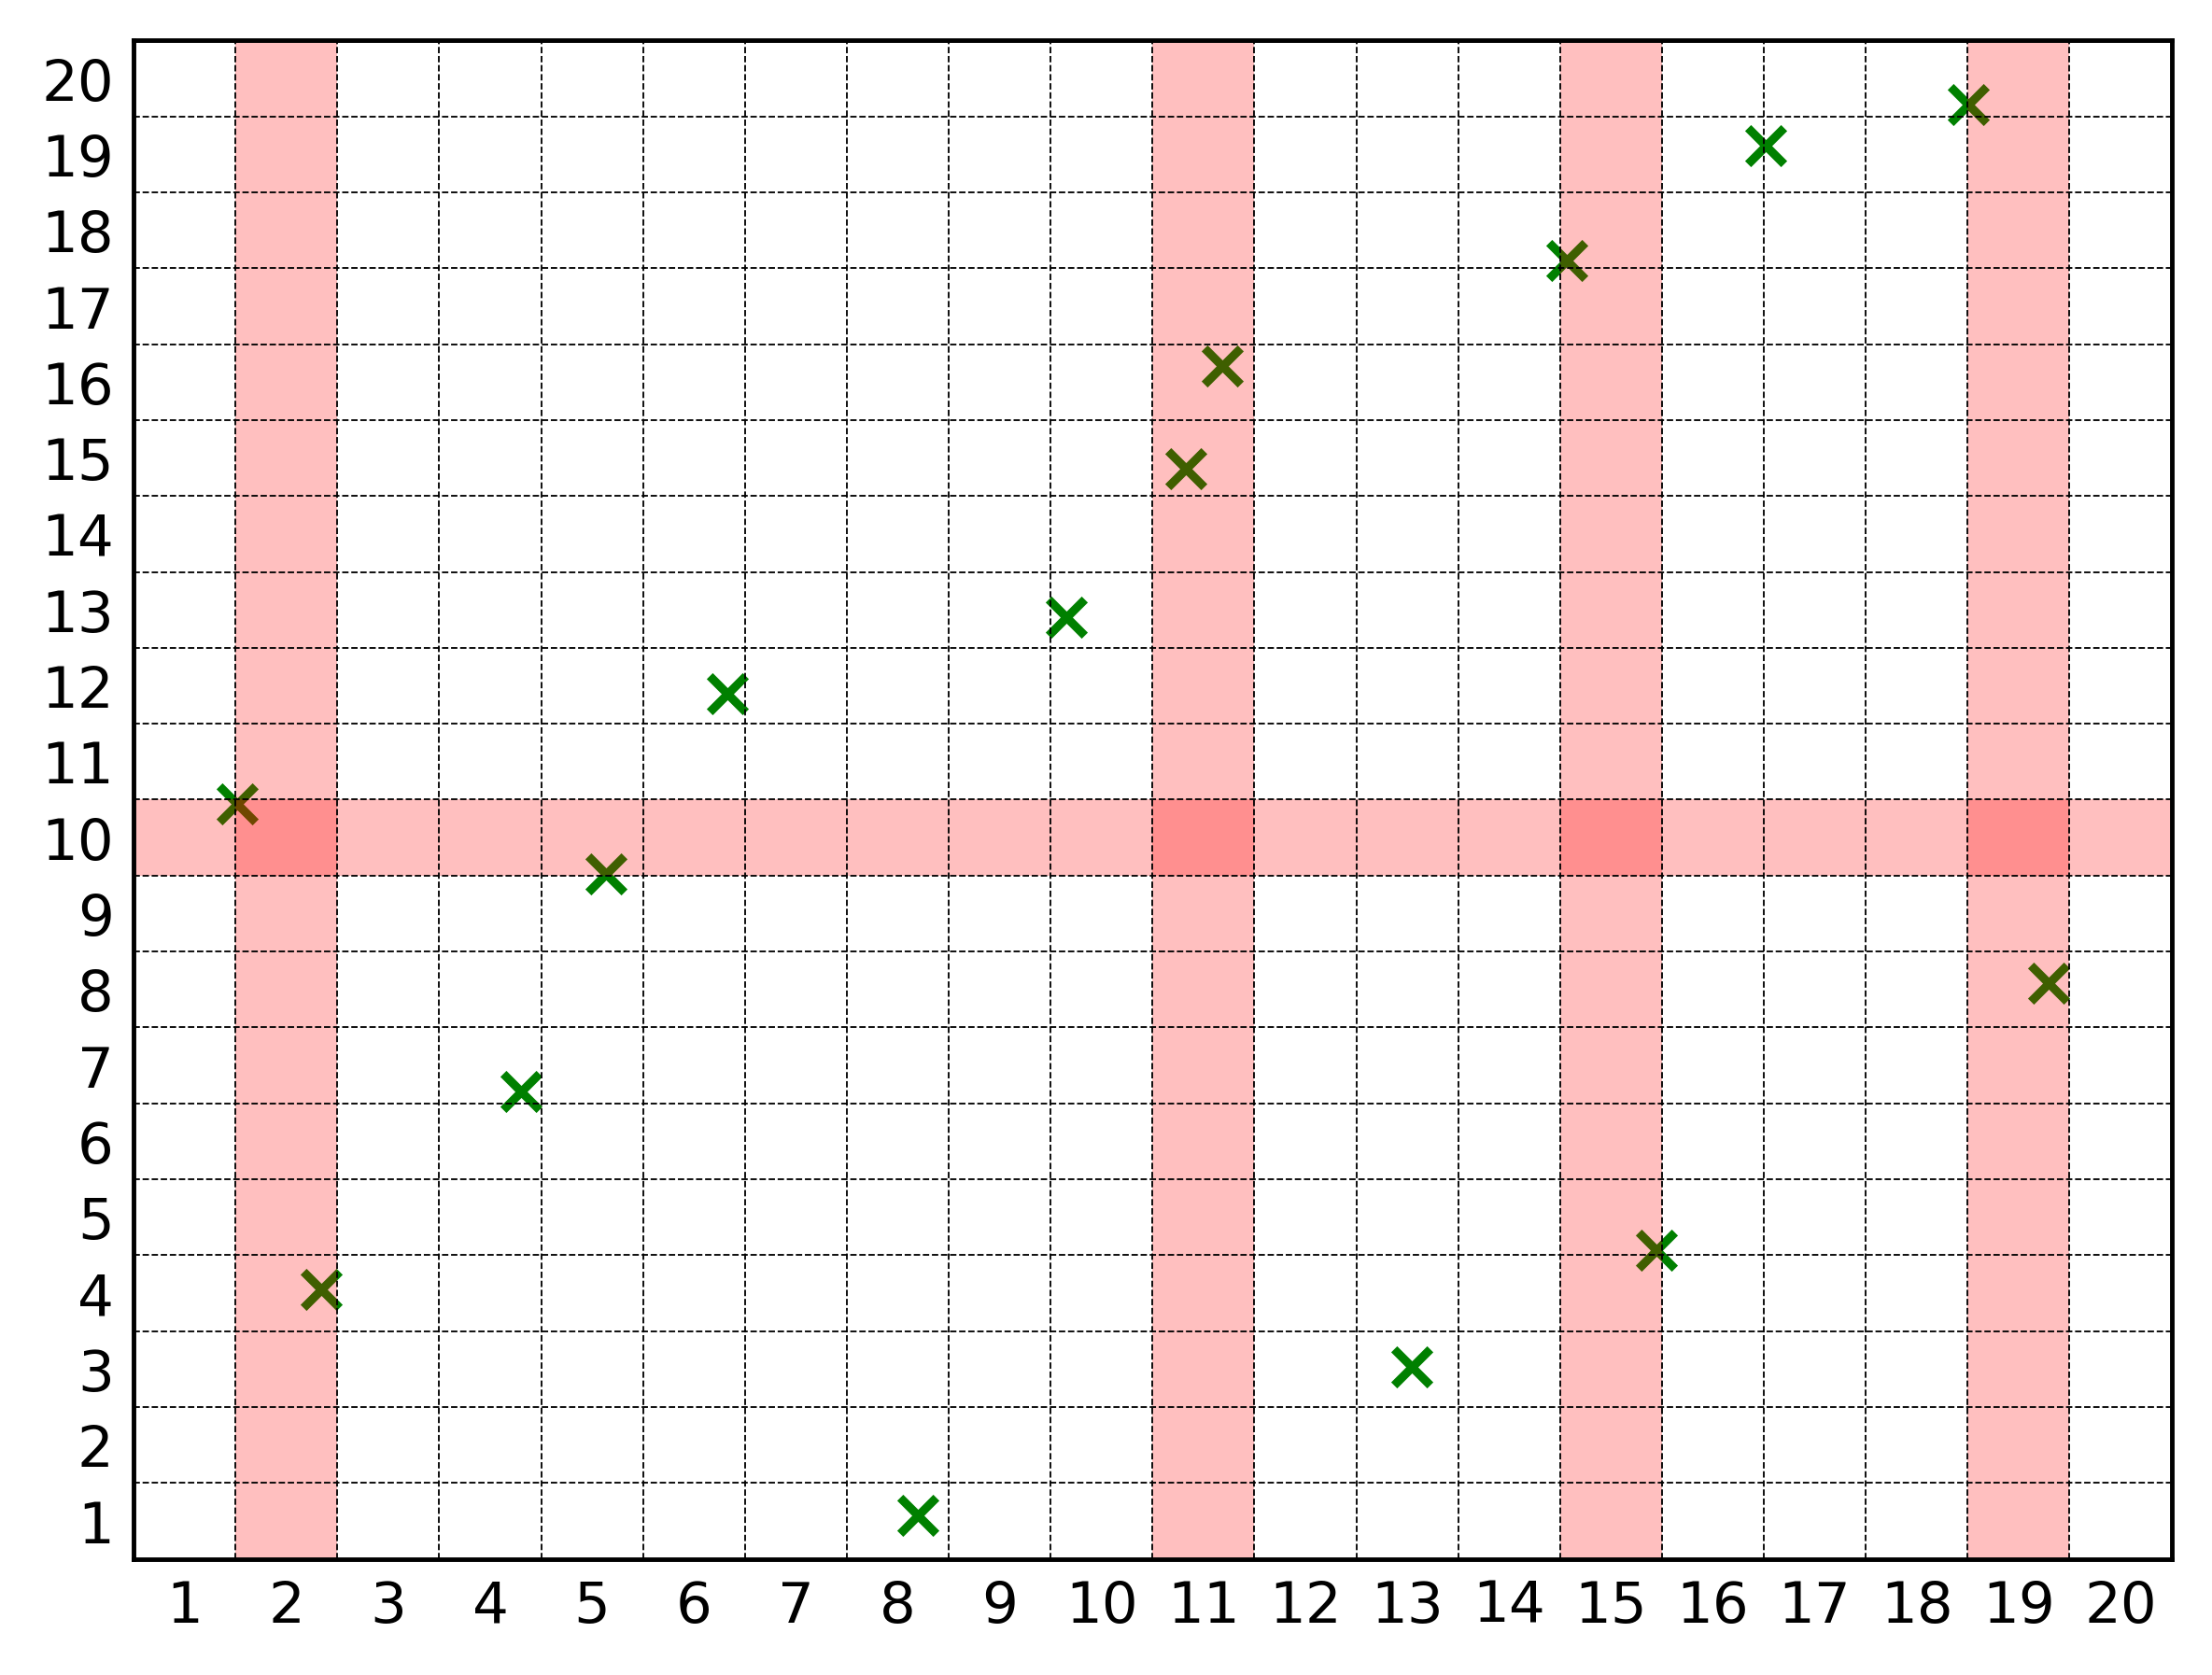
\includegraphics[width=\textwidth]{src/imgs/algo2.png}
        	\captionsetup{skip=0pt}
        	\caption{Red intervals have two sample's projections in it and reduce the space stratification.}
        	\label{fig:algo3}
        }
    \end{subfigure}
    \hspace{0.05\textwidth}
    \begin{subfigure}[b]{0.45\textwidth}
        \centering
        \vtop{
        	\vspace{0pt}
        	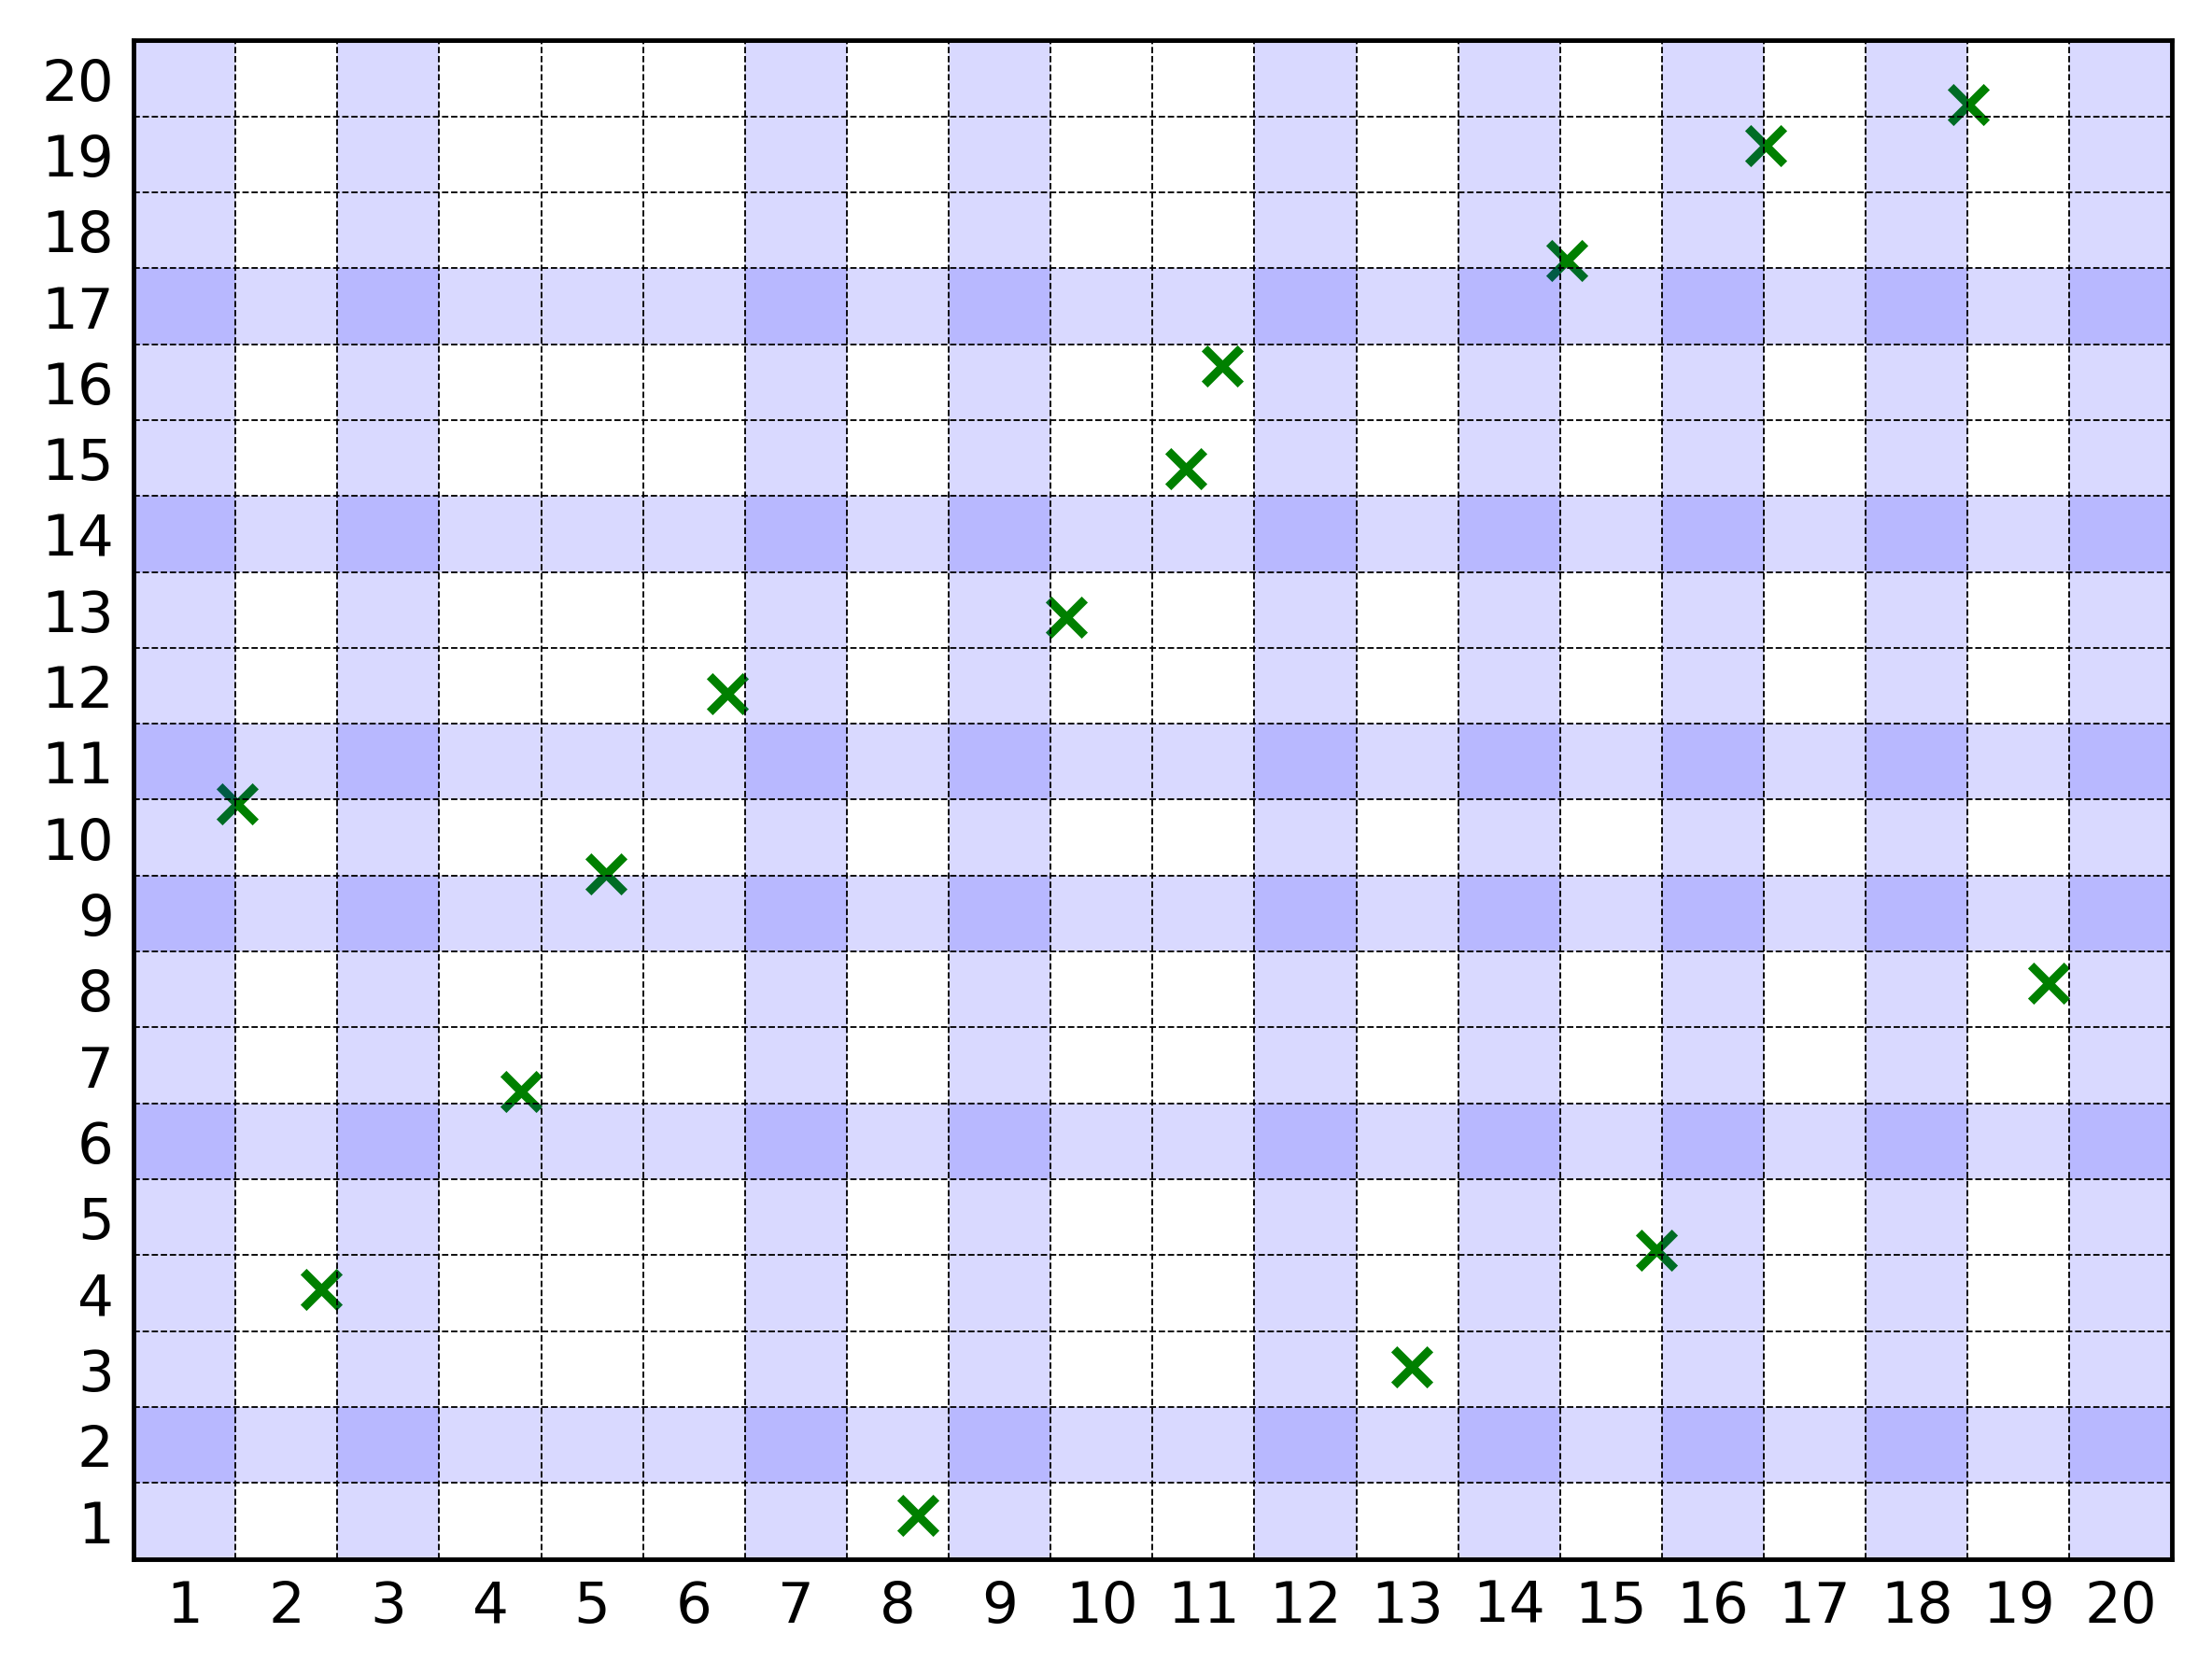
\includegraphics[width=\textwidth]{src/imgs/algo3.png}
        	\captionsetup{skip=0pt}
        	\caption{Blue intervals are empty. They represents the best candidate spots to place new LHS samples. Every interval all together has been referred as the sub-hyperspace of vacancies. }
        	\label{fig:algo4}
        }
    \end{subfigure}

    \captionsetup{justification=centering}
    \caption*{Re-binned (a)'s grid with $N + M$ intervals and plotted against the starting LHS.}
    
   	\midcaption{}
    \label{fig:algo}
\end{figure}

\subsubsection{The eLHS algorithm}
\label{subsubsec:algorithm}
The LHS expansion algorithm, namely \textit{eLHS}, pushes a starting Latin Hypercube $S$ to the next stage $Z = eLHS(S, M)$ by maximizing the hyperspace stratification at most, along with other eventual criterions.

\begin{enumerate}
\item Instance a $V$ vacancies set of $P$ tuples - which may have different lengths (\meqref{eq:voids_matrix}) because every dimension has an arbitrary number of voids (\meqref{eq:vjojm}). The list of all indexes of the $N+M$ grid is filtered accordingly with \meqref{eq:voids_matrix}. \\ 
Visually, the algorithm re-bins the original $S$ grid to achieve $N+M$ intervals. By plotting it against $S$, the reader can visualize where samples overlap and where there are voids.

\item Reduce $V$ vancancies set to a suitable indexes matrix $V^\prime \in Matrix(P, M)$ by extracting from each $\textbf{V}_j$ tuple $M$ elements - which are going to compose the expansion binning grid - using $\sigma$ reduction criteria (see \cref{subsubsec:perfect_expansion_case}). If there are no overlaps (meaning $S$ has maximum expanded degree \meqref{eq:upper_limit_perfect_expansion}) then $V$ is implicitly equal to matrix $V^\prime$, so no reduction criterion is required to be applied. \\
We propose a paradigm which $\sigma$ can be built on. Reduce (abuse of notation) the issue to an harder problem with integer constraints so that solutions are the void interval's indexes. Before generating optimal samples (in step 3.), select the optimal void intervals by considering a trivial "puppet" sample that lies in each possible combination of void intervals. Then apply Branch{\&}Bound methodology [TODO: find good refs for BnB] to find the best integer solution(s).

\item Generate new points over the sub-hyperspace outlined by the permuted $V^\prime$ indexes matrix. Currently, Scipy does not implement the instancing of a LHS over a discontinuous space yet.\\
The eLHS' implementers should achieve drawing optimal data from a discontinuous space on their own, based on desired additional criteria and time complexity requirements. However, we suggest the following algorithm structures.
	
\begin{enumerate}
	\item This procedure was inspired by Shang et al.\ucite{shang2021} work based on the pioneering CADEX research (\fancycite{kennard1969}). It was designed to be fast and flexible given some appropriate criteria to optimize:
	\begin{enumerate}

		\item set the variable $\Lambda = M$, iteration index $k = 1$ and initialize the expanded set $E$ empty;

		\item generate $\Gamma_k$ a random pool of, let's say, $\alpha_k$ number of new random sample points. The hyper-parameter $\alpha_k$ should be much greater than $\Lambda$. We would recommend a fast-and-reliable MCS;
	
		\item ignore all points that fall outside $V^\prime$ space;

		\item from $\Gamma_k$ select a subset of optimal samples $\gamma_k$ of $\lambda_k \leq \Lambda$ number of points.
	
		\begin{enumerate}
			\item[$\dagger$] If $\lambda_k = 1$ it is like drawing the very optimal point each iteration;
			\item[$\dagger$] If $\lambda_k > 1$ the algorithm should yield a bunch of samples which satisfies or optimize any eventual sub-property. Definitely, the basic rule that $\gamma_k$ has to satisfy is the non-collapsing property after being joined with $S \cup E$;
		\end{enumerate}
	
		\item pop out from $V^\prime$ the intervals where $gamma_k$ elements lie in;
	
		\item append the optimal subset: the sample set $E = E \; \cup \;\gamma_k$;
	
		\item set $\Lambda = \Lambda - \lambda_k$. \\
		If $\Lambda = 0$, return $E$. \\
		Otherwise, set $k = k + 1$ and go to step (ii).

	\end{enumerate}
	
	\item The other way to generate $E$ recalls what was said in \cref{subsec:lhs_properties} [not said yet, I'll do it] about search trees. Indeed, as many sampling methods implementations adopt, use a search tree enhances any desired criteria by a lot but trade-offs with time complexity. \\
	However, following there are some further suggestions that the authors have considered notable:
	\begin{enumerate}
		\item A basic search three, branches take a random not yet used vacant space from $V^\prime$ (a $P$ tuple of intervals for each dimension) and shoot $K$ samples, then selects whose the optimal. The deeper the tree goes, the higher is the number of samples drawn. On the leaves there are every expansion sets $E$ computed, the number of leaves is $(M!)^P$. The time complexity is $O\big( K^M \cdot (M!)^P\big)$. This search tree should came along with a reasonable branch pruning rule that reduces computational time and approximate the optimal solution.
		
		\item If multiple criterions are given, build a multi-agent adversarial search algorithm [drop some references from AI here] where each agent (one for each property) tries to optimize its own criteria against the other's (without compromising the global score, the actual objective function linear composed by every criteria).
	
	\end{enumerate}
\end{enumerate}
\end{enumerate}


\section{Examples}
\label{sec:experiments}
This section seeks to evaluate eLHS' sampling performance against other common options, beyond other use cases of the algorithm we have proposed. Specifically, we adopt the classic Monte-Carlo Sampling in the role of mark the performance lower limit whereof other methods might not exceed. In fact, pure MCS is widely deemed as a very poor sampling procedure of an hyperspace \ucite{song2023}. On the other hand, Sobol' are a type of low-discrepancy sequences (for specific details, see \mappendixref{appendix:low_discrepancy}), whose optimality on the topic of sensitivity analysis was observed, rather than LHS \ucite{renardy2021}, and suitable for singular integrals evaluation \ucite{owen1998}. Scipy's implementation (\emph{scipy.stats.qmc.Sobol}) adopts a pre-computed list of base direction numbers (\fancycite{sobol2011}) which act as generative seeds. Furthermore, the Python class \emph{scipy.stats.qmc.LatinHypercube} - LHS sample set generator used in this paper - adopts low-discrepancy optimization criteria along with non-overlapping property. In the end, the Monte-Carlo generator used belongs to Numpy's \emph{numpy.random} utility package, the specific method is \emph{numpy.random.rand} .

The experiments were designed to explore two different important sides of the expansion task, beyond the proposed algorithm:

\begin{enumerate}
\item[(1)] The expected performance of $E$ expanded set, descendant of an LHS, with number of samples $N_{tot} = N_{init} + \sum{M_e}$, should be at least \textit{comparable} with another different standard $S$ Latin Hypercube sample set with same number of samples $N_{tot}$ and built with coherent criteria. The actual performances of the $E$ should be determined only by the effectiveness of the properties, as usual, and do not wane as the evolution proceeds. 

\item[(2)] The expansion process gives the experimenters a new dimension for developing sampling algorithms. Govern the expansion stages may unleash inner properties and high simulation performances that are hard to replicate with monolithic techniques.
\end{enumerate}

Along this section, we will refer to the above sentences as Reason (1) and Reason (2).

The evolution procedure that we used for every example that involves a growing number of samples is different for some experimental set. First of all, a eLHS sample set is deployed as an LHS in first place, then, at each new iteration a brand new expansion is provided, built on the very initial sample set. \\
A variant of this first experimental eLHS is considered. On this scope, the evolution does not descend from the very initial LHS anymore, instead it is cumulative: at each iteration the samples generated during the previous stage works as new starting set. So, when the simulation advances, the samples are "Forwarded" to the next stage, namely \textit{eLHS-F}. In the writers opinion, while eLHS experimental set is the pure essence of how a sole expansion stage behaves, eLHS-F represents the very "applied use" of the algorithm: if, during a simulation, an expansion is needed most likely many more are coming along with it.\\
Sobol' sequences, MC sets and for some LHS sets the expansion paradigm is ruled by adding a fixed number of random samples across the space, without any other specification. The reason for such a trivial expansion is introduced in \cref{sec:introduction}, briefly: we, the authors, aims to evolve an ongoing simulation which, for instance, has not achieved error requirements or we want only spend a limited more computational time at some extent. Obviously, treating an expansion of Sobol', MC or LHS as a whole new simulation with brand new data does not fit with our perspective.

We highlight that some example results are the arithmetic average of a fixed bunch others of equal parameters, so-called agents. This was done because of the high variance of the results detected during the simulations. Take into account that eLHS, eLHS-F and LHS are all based on the same initial Latin Hypercube sample set, then the respective expansion can be deemed as branch choices of the same sample set.

The eLHS software used was implemented by the authors \cref{sec:code_implementation} following the guidelines in \cref{subsubsec:the_algorithm} whereof $\sigma$ functions randomly pops vacancies out the voids set. The optimal search criteria adopted is pure maximin distance of the whole expanded set. The optimal solution is pulled out from a pool of $K = 10$ acceptable expansions. Clearly, such an implementation is trivial and improvable, pondered over time complexity limits assumed and to embrace a real criterion augmentation sufficiently considered for the sake of this paper.

\pagebreak
\subsection{Example I - Stratification evolution}
\label{subsec:exp1}
An important topic of this research was about how to preserve stratification while the sampling evolves. To give an experimental observation about the trend of the degree metric function - again, which quantify the non-overlapping property - a sample set pool has been instanced in first place, then the sample is grown by a step factor equal to 5. 

\mfigref{fig:exp1} depicts 3 scenario with increasing dimension number $P$ equals to 2, 5 and 100. On the horizontal axis varies the $M$ expansion number of samples, on the vertical axis is plotted the result of $\mathcal{D}(S, M)$ for each sample set. The initial sample size is $N = 500$ . Whatever a curve touches the upper stratification heuristic limit 1.0 means that the expanded set at the given $M$ is a perfect expansion.

In the scope of eLHS: for every scenario, we have confirmed experimentally what \meqref{eq:known_perfect_expansions} stress: for each multiple of $N$, the eLHS expansion of any $S$ is perfect. \\
The curve also shows that growing the initial LHS with a relatively small $M$ drops the stratification index by approximately 17\% . This evidence tell us that expansion should be held by almost doubling the sample space, at least.

Unexpectedly, eLHS plot shows evidence of other \textit{peculiar} values of $M$, not yet identified, that seem to optimize stratification locally. Those points occur in every LHS based experimental setup (eLHS, eLHS-F and LHS) at $M \simeq \frac{N}{2}$ and for all $P$ setup. Then, we observed other, less relevant peaks around $M \simeq \frac{N}{4}$ and $M \simeq 2N$. The behavior might suggest a fractal pattern in the degree distribution probability. Such a feature might be matter of further researches.

eLHS-F behavior differs from eLHS because of what we stressed earlier: for small $M$s, it does not worth to expand at all. eLHS-F - that expands the previous expanded set by 5 at each iteration - drops suddenly to around 83\% of stratification and then it is keeping decrease until stationing at 81\% . In order to, underline the importance of the growing step, we will keep the non-optimal step size for eLHS-F next applications.

Sobol' sequences and LHS samples are completely unable to prevent stratification collapse, approaching Monte-Carlo results, which poor performed the tests at every step and bottom limit the simulation. So, unguided Sobol' and LHS both will converge to a Monte-Carlo performance at a swift rate which even increase with dimension. \\ 
Notice that Sobol' and LHS trend to converge. This could suggest how Scipy's produce both: LHS sets are generated from precomputed direction numbers as Sobol' do, then the software filter for those optimized sequences which are Latin Hypercube also. Then Scipy's might be LHS and quasi-Sobol' as well. Disrupting stratification by adding random points each step compromises the non-overlapping property, then the former LHS sets would drop as Sobol' sequences do.


\begin{figure}[H]
    \centering
    \begin{subfigure}[a]{1\textwidth}
        \centering
        \vtop{
        	\vspace{0pt}
        	\includegraphics[width=\textwidth]{../data/plots/exp1.1.P_2.png}
        }
    \end{subfigure}
    \begin{subfigure}[b]{1\textwidth}
        \centering
        \vtop{
        	\vspace{0pt}
        	\includegraphics[width=\textwidth]{../data/plots/exp1.1.P_5.png}
        }
    \end{subfigure}
\end{figure}
\begin{figure}  
    \begin{subfigure}[c]{1\textwidth}
        \centering
        \includegraphics[width=\textwidth]{../data/plots/exp1.1.P_100.png}
    \end{subfigure}
    \midcaption{}
    \label{fig:exp1}
\end{figure}



\subsubsection{Stratification across dimensions}
In \mfigref{fig:exp1_dimensions3} is plotted the same degree function depicted in \mfigref{fig:exp1} but considering all dimension $P$ between 2 and 50. Then it was sectioned 10 times at $M$ equally spaced. The projected sections are shown in \mfigref{fig:exp1_dimensions1} as long as their prime derivative \mfigref{fig:exp1_dimensions2}. 

The example confirms that even for higher-dimensions sample sets, the mean of stratification at fixed $M$s is stationary, meanwhile the variance is effected.

We can conclude that stratification is not effected from $P$ dimensions, but in higher-dimensions the degree is more stable.

\begin{figure}[H]
    \centering
    \begin{subfigure}[b]{1\textwidth}
        \centering
        \vtop{
        	\vspace{0pt}
        	\label{fig:exp1_dimensions1}
        	\includegraphics[width=\textwidth]{../data/plots/exp1.3.M_section.P_2_to_50.png}
        }
    \end{subfigure}
    \begin{subfigure}[b]{1\textwidth}
        \centering
        \vtop{
        	\vspace{0pt}
        	\label{fig:exp1_dimensions2}
        	\includegraphics[width=\textwidth]{../data/plots/exp1.3.M_section_prime.P_2_to_50.png}
        }
    \end{subfigure}
\end{figure}
\begin{figure}
    \begin{subfigure}[b]{1\textwidth}
        \centering
        \vtop{
        	\vspace{0pt}
        	\includegraphics[width=\textwidth]{../data/plots/exp1.3.P_2_to_50.png}
        	\label{fig:exp1_dimensions3}
        }
    \end{subfigure}
    \captionsetup{skip=0pt}
    \caption{The function $\mathcal{D}$(LHS($N$, $P$), $M$) with $P$ and $M$ variables and $N = 500$ is shown in (c). 10 equally spaced sections were taken perpendicular to $M$ and parallel to $P$ (a).  Prime derivatives for each $M$ section in (b)}
    \label{fig:exp1_dimensions}

\end{figure}

\subsection{Example II - Properties mutation}
\label{subsec:exp2}
The aim of this investigation is to test how much the implemented eLHS with its the criteria embedded - which is maximize the minimum distance between sample points - effects the whole sample set. The example wants to empathize how much good new samples are a key aspect to seriously take into account.

The criteria involved are space-filling maximin distance and L2-star discrepancy (\mfigref{fig:exp2}). In first place, every sample set involved is optimized to have good discrepancy properties. Then, during the expansion process, both eLHS and eLHS-F bears new samples with space-filling properties, meanwhile both Sobol and LHS are expanded with Monte-Carlo sample points.

\begin{figure}[H]
    \centering
    \begin{subfigure}[a]{1\textwidth}
        \centering
        \vtop{
        	\vspace{0pt}
        	\includegraphics[width=\textwidth]{../data/plots/exp4.1.mindistance.P_2.png}
        	\label{fig:exp2_spacefilling}
        }
    \end{subfigure}
    \begin{subfigure}[b]{1\textwidth}
        \centering
        \vtop{
        	\vspace{0pt}
        	\includegraphics[width=\textwidth]{../data/plots/exp4.2.discrepancy.P_2.png}
        	\label{fig:exp2_lowdiscrepancy}
        }
    \end{subfigure}
    \captionsetup{skip=0pt}
    \midcaption{}
    \label{fig:exp2}
\end{figure}

There is evidence that both eLHS and eLHS-F outperform the unguided expansion scheme by far regarding maximin distance and minimizing L2-star discrepancy. The characteristic step function is due to the initial sample sets, which have definite minimum distance of fixed points, hence the expanded sets cannot improve it. At least it cannot worsen it. The initial minimum distance represents the upper bound for space-filling optimization search. Despite what observed in what is stressed in \cref{subsec:exp1} about the demoting degree of eLHS-F with respect on the optimal eLHS, the space-filling property does not manifest any relevant disrupting, instead, the minimum distance metric is more stable than eLHS's. 

On the other hand, Sobol' and LHS's discrepancy is outperformed as well, even if the eLHS software was not designed to improve that. Discrepancy performance is relevant in the subjcect of sensitivity analysis, topic of \cref{subsec:exp3}.

This investigation shows the potential of expansion process on the every properties of a sample set. In the matter of Reason (2), the initial eLHS and eLHS-F have achieved a better discrepancy and space-filling properties than the optimal experimental setups Sobol' and standard LHS enriched with trivial Monte-Carlo sample points.


\subsection{Example III - Expansion of Monte Carlo Integration}
\label{subsec:exp3}
In the scope of this example, the Monte-Carlo integration adopts a quasi-MC sample distribution to compute numerically the integral of the multivariate function:
%np.exp(-x**2 - y**2 - z**2) * np.sin(x) * np.cos(y) * np.sin(z)
\begin{equation*}
f(x,y,z) = e^{-x^2-y^2-z^2} \cdot sin(x) \cdot cos(y) \cdot sin(z)
\end{equation*}
on the integration interval $[0, 1]^3$ .
For technical formulation of this technique and how it is applied to carry out the simulation, please refer to \mappendixref{appendix:montecarlo_integration} .

The growing step is set to 50, the total number of samples ranges from 100 to 10000. The total number of agents is 10. 
All experimental setups share the same initial LHS sets.

\mfigref{fig:exp3_error} depicts absolute error evolution throughout simulation expansions. Instead, \mfigref{fig:exp3_time} shows the computational time measured at the end of every step. The experimental sets are eLHS-F and eLHS as usual and the Random-LHS distribution, which is a sample set pool pulls out a new sample set at each step. Random-LHS was adopted to simulate what the experimenter should expect if, for instance, the MC integration does not satisfy the maximum error requirement (or any other) and thus they decide to redeploy the whole simulation by creating a new sample set with increased sample size. This kind of expansion pool is in direct contrast with the assumption stated in \cref{sec:experiments}. That's because the below tests can justify Reason (1). 

The high-precision result of the integral which the outcomes have been compared to is yielded by \emph{scipy.integrate.nquad} adaptive multidimensional integration quadrature method. The resultant error is the absolute difference between the deployed MC Integration over the handed sample set and Scipy's result.


\begin{figure}[H]
    \centering
    \begin{subfigure}[a]{1\textwidth}
        \centering
        \vtop{
        	\vspace{0pt}
        	\includegraphics[width=\textwidth]{../data/plots/exp2.mcaccuracy.N_100_to_10000.v2.png}
        	\label{fig:exp2_spacefilling}
        }
    \end{subfigure}
    \begin{subfigure}[b]{1\textwidth}
        \centering
        \vtop{
        	\vspace{0pt}
        	\includegraphics[width=\textwidth]{../data/plots/exp2.mctime.N_100_to_10000.v2.png}
        	\label{fig:exp2_lowdiscrepancy}
        }
    \end{subfigure}
    \captionsetup{skip=0pt}
    \midcaption{The example was ran on a single unit Macbook Air (2020), CPU/GPU: Silicon M1}
    \label{fig:exp2}
\end{figure}

The discrepancy in the earlier stages of evolution between eLHS and eLHS-F is justified by the Monte-Carlo integration's high variance predictions. On the other hand, eLHS keeps the error rate comparable to Random-LHS.\\
By stressing this, we have fulfilled Reason (1) requirements: eLHS and LHS are yet comparable and, in this specific case study, the former outperforms the latter.

eLHS-F close perform the other ones but never exceeding them, the reason is linked to the observation in \cref{subsec:exp1}. In the first-stage, the fixed step expansion size (50) is equal to the 50\% of the initial sample size (100); on the second-stage, the ratio $\frac{M}{N}$ drops to 33\%, then 25\%, 20\% etc. So, stratification consistency does not hold as well as it should do. Hence, accuracy performance trade-offs with execution time.

On the computational time, the authors achieved a so less execution effort using eLHS-F because the experimental setup is affected by the numerical Monte-Carlo integration next-step rule (\meqref{eq:mc_next_step}).


\section{Code implementation}
\label{sec:code_implementation}
In this section, the code implementation of eLHS algorithm and degree function is shown and commented. 

The interface language is Python 3.1 and later versions, widely used among scientist and lender of many very advanced mathematics libraries and optimized data structures. While dealing with large bunch of data, it is recommended to develop their own software solution using C/C++ programming languages. By default, Python exports API for porting C language, distributed with Python.h header file. Python APIs are not subject of this research, although it may happen that some code refer to owned Python data structures. The developed C module file for Python has been compiled using clang 15.0.0 (clang-1500.3.9.4) stable release. Furthermore, the flag \emph{-fno-vectorize} for clang compiler has been enable to cast loop vectorization on a data vector with variable width, decided on compile time by a cost model evaluation on computational resources available and cost of memory write outs \ucite{vectorization}.

Future versions would implement parallelization with pthreads to optimize large data structure CRUD operations and concurrent search trees. We do also have assessed that the algorithm could be reorganized to better match Superword-Level-Parallelism (SPL) prerequisites which is incompatible with loop vectorization by LLVM project.

The full project code is publicly available online and ruled by MIT License on my personal GitHub respository: \url{github.com/alecrespi/PLHS} . The package will be distributed with Python package manager \emph{pip} under the name of \emph{latinexpansion}.


\subsection{eLHS - Expansion Algorithm}
\label{subsec:eLHS_code}
The software was implemented accordingly with guidelines in \cref{subsubsec:algorithm}.

The Python function signature is:

\begin{lstlisting}[language=Python]
def eLHS(S:numpy.ndarray, M:int, throws:int = 10) -> numpy.ndarray
\end{lstlisting}

The \emph{vacancies{\_}list} struct type has been used to build the irregular set of tuples referred as $V$ throughout this paper. It tracks down how many vacancies has been found in a specific dimension. A tuple (array) of integers indexes of the same size is allocated. Definition:

\begin{lstlisting}[style=CStyle]
typedef struct vlist{
    int len;
    int* vacancies;
} vacancies_list;
\end{lstlisting}

To enhance code readability, some pre-processor macros have been defined as well:

\begin{lstlisting}[style=CStyle]
// given q interval index, get interval lower bound
#define I(q) (((double)q)/(N+M))     

// given x sample, get its interval index
#define Q(x) (floor(((double)x)*(N+M)))     

// var swapping, do-while block triggers pre-processor 
// multi-line rescripting
#define SWAP(a, b) do { typeof(a) tmp = a; a = b; b = tmp; } while (0)  

// given q interval index, generate a random sample in it 
#define R(q) ((double)I(q) + ((double)rand()*I(1) / RAND_MAX))

\end{lstlisting}

The variable identifiers are
\begin{enumerate}
\item[] \emph{N, M, P} $\rightarrow$ number of samples in ss, number of additional points, number of dimensions. All strictly positive.

\item[] \emph{ss} $\rightarrow$ shorthand for \textit{sample set}, $N \times P$ matrix of double;

\item[] \emph{exp} $\rightarrow$ shorthand for \textit{expansion set}, $M \times P$ matrix of double;

\item[] \emph{vs} $\rightarrow$ shorthand for \textit{vacancies set}, $P$-long array of \textit{vacancies{\_}list} structs;

\item[] \emph{v{\_}prime} $\rightarrow$ the $V^\prime$ vacancies matrix, $M \times P$ matrix of integers;
\end{enumerate}

The C core body module of eLHS is given below:
\begin{lstlisting}[style=CStyle]
static PyObject* method_eLHS (...) {
	// variable declaration block
    double max_distance = 0.0;
	// interface with Python.h API
	...
	// getting the whole vacancies 
    vs = build_vacancies_matrix(ss, N, P, M);

	/* try `throws` times to keep maximin distance optimal */
    for(t = 0; t < throws; t++){
        /* shuffle and subset vacancies set at each iteration */
        v_prime = shuffle_subset_vacancies(vs, M, P);
        
        // sowing new points
        for(i = 0; i < M; i++)
            for(j = 0; j < P; j++)
                exp[i][j] = R(v_prime[j][i]);
        
	    // maximin distance search 
        if(throws != 1){
            dist = min_distance(ss, exp, N, M, P);
            if(dist > max_distance)
                max_distance = dist;
        }
    }
    ...
	// returning exp PyObject* data struct as eLHS result
}
\end{lstlisting}


The core module in C is then subdivided in the following 4 macro routines. 

\subsubsection{build{\_}vacancies{\_}matrix}
The first step of the algorithm is to track down every vacant interval in every dimension. Thus, 

\begin{lstlisting}[style=CStyle]
vacancies_list* build_vacancies_matrix
	(double** ss, int N, int P, int M)
{
    vacancies_list *vs;
    int i, j, q;

    vs = (vacancies_list*)malloc(P*sizeof(vacancies_list));

    for(j = 0; j < P; j++){
        int vindex = 0;
        int *vptr = (int*) malloc((N+M)*sizeof(int));
        // masks vptr elements if they are void 
        bool *vmask = (bool*) malloc((N+M)*sizeof(bool));   
        // set mask to false 
        memset(vmask, 0, (N + M) * sizeof(bool));           
        
        // map down the busy intervals (busy is TRUE)
        for(i = 0; i < N; i++)
            vmask[(int) Q(ss[i][j])] = true;
        
        // mask the interval indexes to gather only voids
        for(q = 0; q < N+M; q++){
            // if q is a void, then add it
            if(!vmask[q])   
                vptr[vindex++] = q;
        }

        // realloc voids sequence to fit void numbers
        vptr = (int*) realloc(vptr, vindex * sizeof(int));
        if(!vptr)   return NULL;
        // build up vacancies_list entry
        vs[j].len = vindex;
        vs[j].vacancies = vptr;
    }
    return vs;
}
\end{lstlisting}


\subsubsection{shuffle{\_}subset{\_}vacancies}
Shuffle the vacancies set \emph{vs} and apply the $\sigma$ criterion chosen. The implementation permutes randomly each vacancy{\_}list array attribute and then cut off the exceeding intervals. 

\begin{lstlisting}[style=CStyle]
int **shuffle_subset_vacancies
	(vacancies_list* vs, int M, int P)
{
    if(!vs || M == 0) return NULL;
    int **v_prime = (int **)malloc(P * sizeof(int*));

    /* for each dimension, shuffle and reshape the vacancy list to a regular size M */
    for(int j = 0; j < P; j++){
        if(!vs[j].vacancies || !vs[j].len)
            return NULL;

        int *vptr = (int*)malloc(vs[j].len * sizeof(int));
        /* copy elements to preserve data integrity for further steps*/
        for(int i = 0; i < vs[j].len; i++)
            vptr[i] = vs[j].vacancies[i];

        /* shuffling all items */
        for (int i = vs[j].len; i > 0; i--){ 
            // generate a random index that ranges from [0, M-1]
            int r = rand() % i;     
            SWAP(vptr[i-1], vptr[r]);
        }
        /* truncate the list to M */
        vptr = (int *)realloc(vptr, M*sizeof(int)); 
        v_prime[j] = vptr;
    }
    return v_prime;
}
\end{lstlisting}

\subsubsection{sample{\_}sowing}
Based on $V^\prime$ shuffled matrix, generate a brand new expansion set and store it in \emph{exp} matrix. This routine is hard coded in the eLHS module body. 

\begin{lstlisting}[style=CStyle]
// in the declaration block
// allocate exp result matrix 
exp = (double **)malloc(M * sizeof(double*));
for(i = 0; i < M; i++)
	exp[i] = (double *)malloc(P * sizeof(double));
...
//sample_sowing
/* for each new sample */
for(i = 0; i < M; i++)
	/* for each dimension */
	for(j = 0; j < P; j++)
		/* generate sample in the random interval v_prime[j][i] */
		exp[i][j] = R(v_prime[j][i]);
...	
\end{lstlisting}

\subsubsection{minimax{\_}search}

\begin{lstlisting}[style=CStyle]
// in the declaration block
double max_distance = 0.0, dist;
...
while (condition){
	...
	dist = min_distance(ss, exp, N, M, P);
	if(dist > max_distance)
		max_distance = dist;
	...
}

// somewhere else in function initialization section
/* computes minimum distance among every points, only expansion points are considered beacuse initial points have fixed minimum distance */
double min_distance
(double **ss, double **exp, int N, int M, int P)
{
    int i, k;
    /* __DBL_MAX__ will force the first minimum if-condition */
    double min = __DBL_MAX__, dist = 0.0;
    
    for(k = 0; k < M; k++){
    	/* search minimum distance among expansion points and initial points */
        for(i = 0; i < N; i++){
        	// P-degree euclidean distance as metric
            dist = euclid(exp[k], ss[i], P);
            if( dist < min ) min = dist;
        }
    	/* search minimum distance among expansion points themselves */
        for(i = k + 1; i < M; i++){
            dist = euclid(exp[k], exp[i], P);
            if( dist < min ) min = dist;
        }
    }
    return min;
}
\end{lstlisting}

\subsection{Degree function - Stratification heuristic}
\label{subsec:degree_code}
The degree heuristic software formally implements \meqref{eq:expanded_degree} definition. It was deployed to carry out \cref{subsec:exp1} Example I simulations.

The Python signature for this method is:
\begin{lstlisting}[style=CStyle]
def degree(S:numpy.ndarray, M:int = 0) -> float
\end{lstlisting}

The function's body follows:
\begin{lstlisting}[style=CStyle]
...
double gr = 0;
// compute degree
for(j = 0; j < P; j++){
    for(q = 0; q < N+M; q++){
        for(i = 0; i < N; i++){
        	/* check if sample's projection lies in q interval */
            if(I(q) <= ss[i][j] && ss[i][j] < I(q+1)){
                gr += 1;
                /* if found, break the samples' loop (simulates `min` operand of the formula */
                break;
            }
        }
    }
}
gr /= (double) P * (N + M);
...
// return PyObject* representing `gr` result
\end{lstlisting}

\section{Conclusions}
\label{sec:conclusions}
The expansion process has demonstrated high capabilities of enhancing an ongoing simulation thanks to the evolutionary analysis that the authors depict. The number of additional points are a crucial variable to ponder: too low $M$s annihilate the original LHS stratification property across the space; instead, higher $M$s, roughly above $N$ - so by doubling the sample size - the accuracy increases and stratification is almost kept but may fail on the computational limits requested.

Expansion may be ruled by a optimization criteria which can differ from the ones which the initial sample set was built on. This heterogeneous mixture of properties can be crucial in solving complex simulation dynamically, by improving a different criteria on the need. Example II (\cref{subsec:exp2}) experimental setups exhibit this flexibility.

The research has also proposed the degree and expanded degree heuristics, along with their properties, which demonstrated to be useful tool for quantify stratification in any quasi-Monte-Carlo sampling. 

Referring to the innovative work of \ucite{sheikholeslami2017} about \textit{Progressive Latin Hypercube Sampling} - which is a theoretical class of sampling methods with adaptive sample size based on intrinsic properties of the sample set - the multistage evolutionary approach that this paper discuss can represent the very fundamental computational aspect of enlarging (or shrinking) the sample set size on the need.

This research allowed the authors to develop and release the first official latinexpansion package for Python API (\fancycite{crespi2024}) that include \textit{expanded degree} stratification metric and \textit{eLHS} expansion algorithm for any sample set.

Research might turn toward the analysis of the probabilistic distribution of the degree stratification index, explaining the optimal stratification spikes observed in Example I (\cref{subsec:exp1}), and looks for an optimal pool of Latin Hypercube sample sets which are best to expand.

\section{APPENDIX}
\label{appendix}
\subsection{Indicator function}
\label{appendix:indicator_function}
The indicator function $\indfunc{}$ of a set \textbf{A} indicates whether the input belongs to $A$ or not, specifically:
\begin{equation}
\label{eq:indicator_function}
\indfunc{A}(x) := 
\begin{cases}
1 \qquad \text{\textit{if x $\in$ A}}\\
0 \qquad \text{\textit{if x $\not\in$ A}}
 \end{cases}
\end{equation}
As in the matter of sectioning a space into continuous intervals in the shape of [a, b), it is useful to redefine the indicator function as an operation that occurs with the boundaries of $A$ using the Heaviside step function which does not involve set operators but only logical ones. It's important to remark that it does not matter what happens precisely on the boundaries. 
The Heaviside function is defined:
\begin{equation}
\label{eq:heaviside}
H(x) := 
\begin{cases}
1 \qquad \text{\textit{if x $\geq$ 0}}\\
0 \qquad \text{\textit{if x $<$ 0}}
\end{cases}
\end{equation}
So the indicator function can be also produced:
\begin{equation}
\label{eq:indicator_function_with_h}
\indfunc{[a,b)}(x) = H(x - a) \cdot H(b - x)
\end{equation}

\subsection{Known perfect expansion explained: Multiples of N}
\label{appendix:N_multiples}
Given $S \in LHS(N, P)$ set with $N, P \in \mathbb{N}$ respectively number of samples and dimensions, by definition (\meqref{eq:degree_of_lhs}), has maximum $\mathcal{D}$ degree. Experimentally, it has been observed that the only well-known perfect expansions (maximum expanded degree \meqref{eq:expanded_degree}) of $S$ are those which the $M$ increment of the sample space is a multiple of $N$ (\fancycite{falcone2023}). Experimental evidences are depicted in \mfigref{fig:exp1}.

The reason of this behavior is linked to the unique distribution characteristic that intervals the $M = K \cdot N$ growing grid and the initial $S$' grid share: the former, actually, sections - with abuse of notation - \emph{perfectly} the latter's intervals space. \textsuperscript{(*)} By considering the same amount of samples $N$ for both situations, we can state that the sum of the shares along any dimension of the regridded set is equal to the initial's one, which is equal to $N$.\\
Let's stress out the degree and expanded degree equations:

\begin{equation*}
\mathcal{D}(S) = \frac{1}{P \cdot N} \cdot \sum^P_{j=1} \sum^N_{q=1} min(\sum^N_{i=1}\indfunc{[\frac{q-1}{N}, \frac{q}{N})}(S_{ij}), 1) = 1
\end{equation*}
\\
the total share of all intervals along a fixed dimension is:

\begin{equation*}
\sum^N_{q=1} min(\sum^N_{i=1}\indfunc{[\frac{q-1}{N}, \frac{q}{N})}(S_{ij}), 1) = N
\end{equation*}

Given the unique property cited above (*), also given $N + M = (K+1) \cdot N $, the expanded grid should have the exact same amount of share:

\begin{equation*}
\sum^{{\scriptscriptstyle (K+1) \cdot N}}_{q=1} min(\sum^{N}_{i=1}\indfunc{[\frac{q-1}{{(K+1) \cdot N}}, \frac{q}{(K+1) \cdot N})}(S_{ij}), 1) = N
\end{equation*}
\\
then, the expanded degree should be:

\begin{equation*}
\mathcal{D}(S, K \cdot N) = \text{\scalebox{0.75}{$\frac{1}{{P \cdot (K+1) \cdot N}}$}} \cdot \sum^P_{j=1}\sum^{{\scriptscriptstyle (K+1) \cdot N}}_{q=1} min(\sum^{N}_{i=1}\indfunc{[\frac{q-1}{{(K+1) \cdot N}}, \frac{q}{(K+1) \cdot N})}(S_{ij}), 1) = \frac{1}{K+1}
\end{equation*}

which corresponds exactly to the upper limit of an $M = K \cdots N$ growing step grid for an $S$ LHS set \meqref{eq:upper_limit_perfect_expansion}: 

\begin{equation*}
\mathcal{D}(S, K \cdot N) = \frac{1}{K+1} = 1 - \frac{K \cdot N}{(K+1) \cdot N} = \mathcal{D}_{max}
\end{equation*}

Hence, any $S$ expansion of $K \cdot N$ magnitude has maximum expanded degree, which makes them \textit{perfect expansions} by definition.

\subsection{Monte-Carlo Integration}
\label{appendix:montecarlo_integration}
Monte-Carlo Integration is a powerful numerical integration technique widely adopted in engineering and physics. It is deployed in high-dimensional spaces where traditional methods become too much computational demanding and the trade-off between computational time and estimating gain become infeasible. Basically, this is a stochastic method where $N$ points are randomly sampled in a parameter space, a so-called Monte-Carlo Sampling. 

Given a $f(\bar{x})$ of $P$ parameters, the integral:
\begin{equation*}
I = \int{\Omega}f(\bar{x})d\bar{x}
\end{equation*}
is approximated by the Monte-Carlo integral:
\begin{equation*}
I \simeq \frac{V}{N} \cdot \sum^N_i{f(\bar{x}_i)}
\end{equation*}

If two quasi-MC sample sets are involved, let's say $X$ and $Y$ of $N_1$ and $N_2$ sample size respectively, the integral take the form:
\begin{equation*}
I = \frac{V}{N_1 + N_2} \cdot \sum^{N_1 + N_2}_i{f(\bar{x}_i)}
\end{equation*}
If $I_1$ integral computed for $X$ is known, then to compute the estimated $I$ is only necessary to compute for $Y$ and combine both using:
\begin{equation}
\label{eq:mc_next_step}
I = \frac{N_1}{N_1 + N_2} \cdot I_1 + \frac{V}{N_1 + N_2}\sum^{N_2}_{i=N_1}{f(\bar{x}_i)}
\end{equation}

\subsection{Low-Discrepancy sequences}
\label{appendix:low_discrepancy}
Low-discrepancy sequences are a class of quasi-MC sampling methods which adopt a discrepancy minimization criteria, a measure of the deviation of the distribution of sample points from uniformity. One commonly used metric for evaluating this uniformity is the L2-star discrepancy, which quantifies how well the sample points cover the integration domain.

Sobol’ sequences are a type of low-discrepancy sequence, developed by \fancycite{sobol1967}, that provides a highly uniform distribution of points in multi-dimensional spaces. They are particularly effective in numerical integration and sensitivity analysis. The construction of Sobol’ sequences involves the use of direction numbers and primitive polynomials to achieve a uniform spread of points \ucite{dick2010}. 

\pagebreak
\printbibliography
\end{document}
